\pagebreak
\section{3D Results}
\add[XT]{add one more section as an individual file/chapter for 2D models description.}
%\subsection{3D model results}
%\add[XT]{choose some points in the model domain like Choi 2008 did, to monitor the values changes with time (e.g. In VisIt use Query to obtain stress with time for quantatatively analyzing the model behaviors)}
Currently, we have three factors controlling the model behaviors. They are three ranges of M variation along the ridge axis (0.5$\sim$0.7; 0.5$\sim$0.8; 0.2$\sim$0.8), three functional forms of M variation (linear; sinusoidal; square root) and two types of weakening rate (Type one and Type two) as described in detail in the section ``Parameters to control''. 

In this ``Results'' chapter, we will first describe in detail the model behaviors of two reference models. Then, we will compare the reference model and the other data points with different setup parameters. %Formation mechanism will be explained mostly in this chapter and will be further discussed and compared with nature observation in the ``Discussion'' chapter. 

\subsection{Reference models (M28LinT1 Table~\hyperref[Tab1_1]{\ref{Tab1_1}})}\label{sec_M28LinT1}

We consider M varies linearly from 0.2 to 0.8 along the ridge axis with increasing Z as our reference model.

\begin{figure}[h]
  \centering
    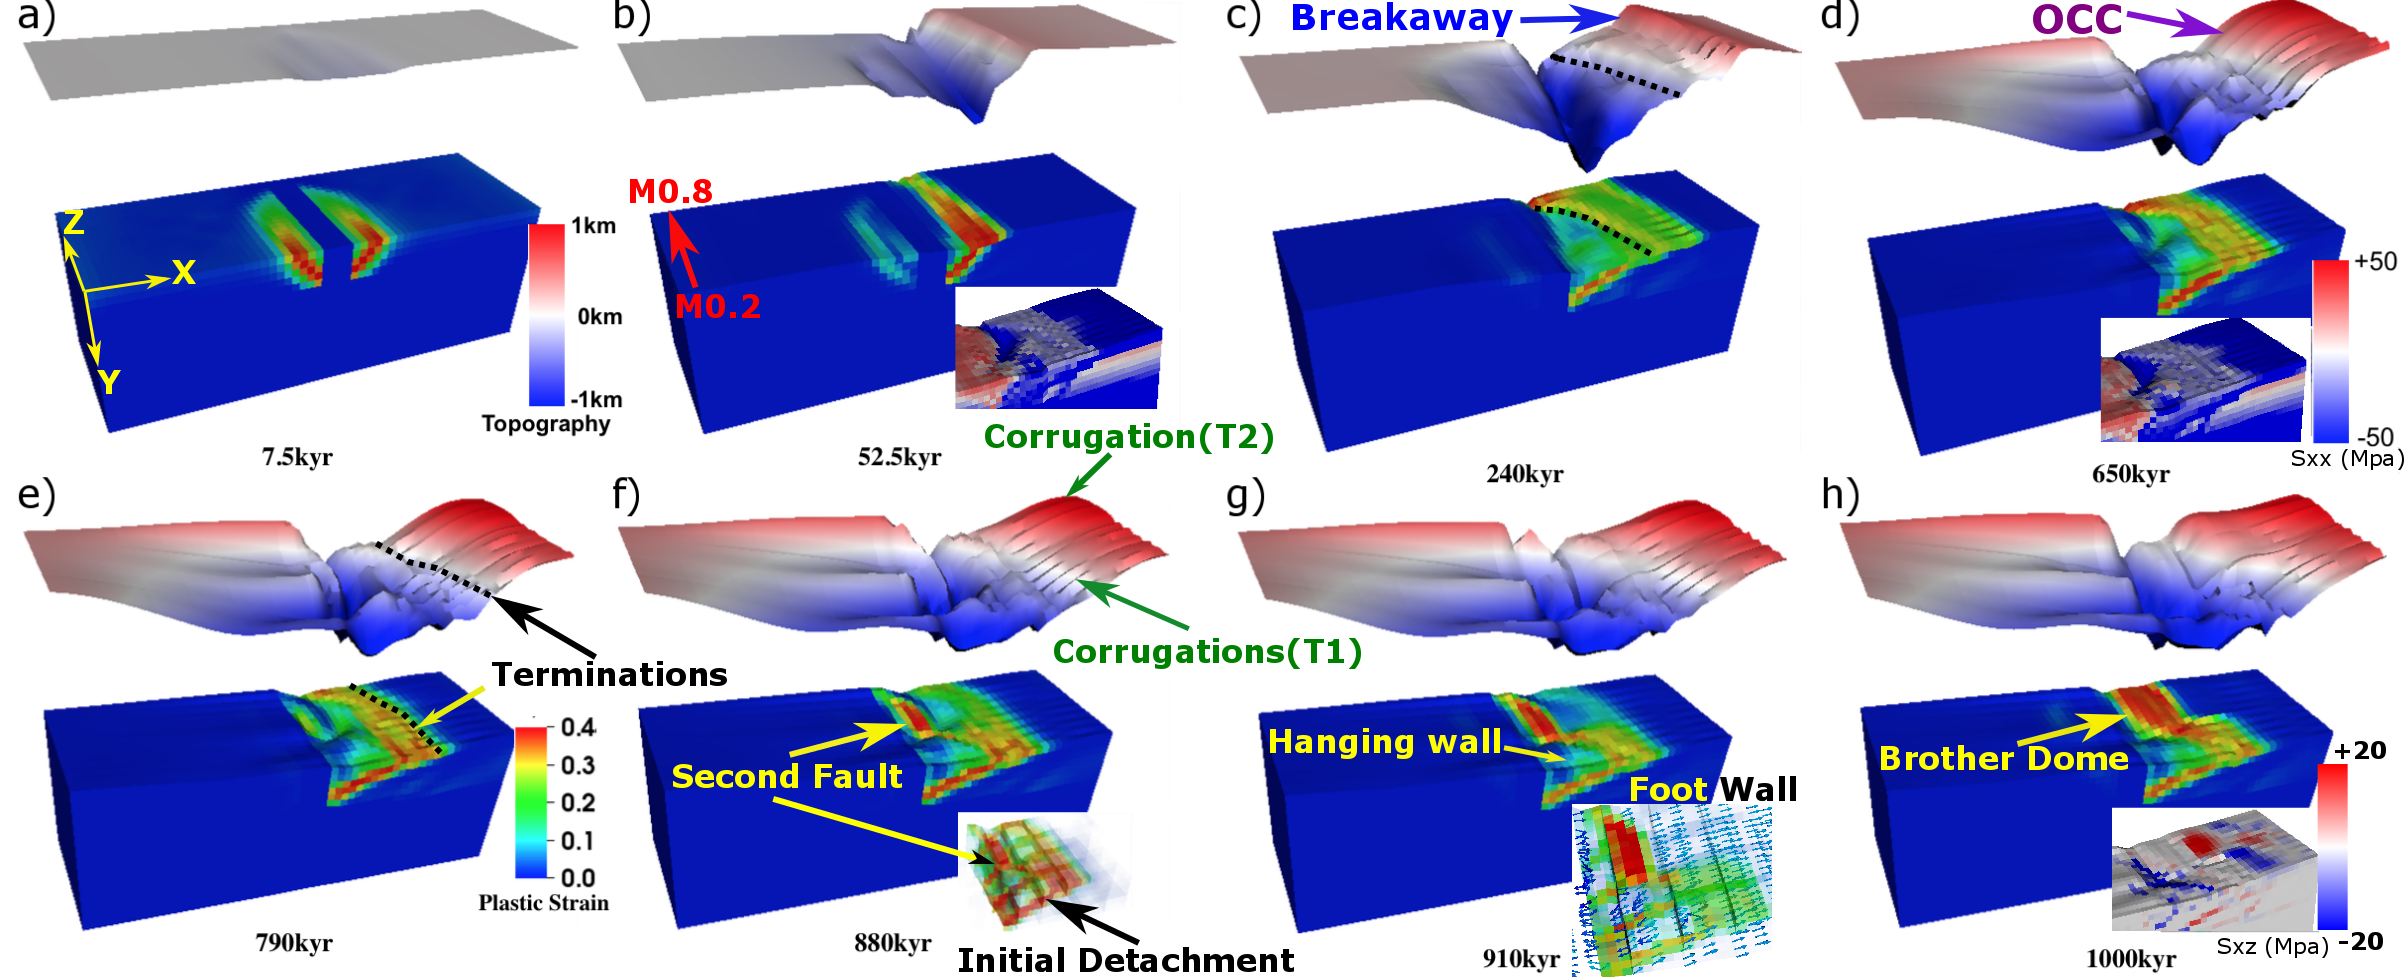
\includegraphics[width=1.0\textwidth]{./Figures/fig_Results1_1.png}
  \caption{Reference model one: M linearly increases from 0.2 to 0.8 from front to back, Type one weakening (M28LinT1) (Table~\hyperref[Tab1_1]{\ref{Tab1_1}}). The top layer is the topography of the model with five times vertical exaggeration. The color scale within Figure~\hyperref[fig_Results1_1]{\ref{fig_Results1_1}.a} is for the topography. Initial seafloor is marked as a reference of zero km in height.  The green, yellow and red colors in the background of blue model domain are plastic strain. Its color scale is shown in Figure~\hyperref[fig_Results1_1]{\ref{fig_Results1_1}.e}. The number with kyr as a unit beneath each model result is the time for the model with a unit of thousands of year. The two insets in Figure~\hyperref[fig_Results1_1]{\ref{fig_Results1_1}.b} and Figure~\hyperref[fig_Results1_1]{\ref{fig_Results1_1}.d} is for stress $\sigma_{xx}$ (Sxx in the figure). Positive value (pink and red) means tension and negative (blue) is compression. The inset in Figure~\hyperref[fig_Results1_1]{\ref{fig_Results1_1}.h} is for shear stress $\sigma_{xz}$ (Sxz in the figure). It share the same color scale with insets in the Figure~\hyperref[fig_Results1_1]{\ref{fig_Results1_1}.b} and Figure~\hyperref[fig_Results1_1]{\ref{fig_Results1_1}.d}. The inset in Figure~\hyperref[fig_Results1_1]{\ref{fig_Results1_1}.f} is a transparent view of plastic strain. The inset in Figure~\hyperref[fig_Results1_1]{\ref{fig_Results1_1}.g} shows both plastic strain and the velocity vector. Indicated by the velocity vector, the hanging wall of the detachment fault at low M region (M0.2$\sim$M0.5) is moving in an opposite direction to the hanging wall at higher M region (M$>0.5$).} %\note[XT]{one thing to be noted is that the $dt=0.5yr$ in these series of 3D models, thus I divided the time step by two to get the time (kyr). This figure needs to be revised that the plastic strain scale is actually changing for different time, a way to revise it is to maintain a constant color scale or attach a color scale for each time. Also, it seems a little bit small and two rows is not as preferable as one row or one column to better express the concept of linear time series evolution.}}
 \label{fig_Results1_1}
\end{figure}   

As shown in Figure~\hyperref[fig_Results1_1]{\ref{fig_Results1_1}}, the model creates a median valley that both widens and deepens through time and the rate of its widening and deepening at a specific location (in terms of Z-axis) is inverse proportional to the rate of local magma supply (i.e. M value). OCCs with more than one kilometer in relief and tens of kilometers in wavelentgh are produced in the model. One interesting behavior worth noting is that corrugations with hundred-to-kilometer wavelengths are also produced by the model.

As shown in Figure~\hyperref[fig_Results1_1]{\ref{fig_Results1_1}.a}, in the first 7.5kyr, high angle ($\sim 60 \degree$)(consistent with  Anderson's theory of faulting mechanics for a frictional angle of 30$\degree$) normal faults (shown as higher plastic strain shear bands with a thickness of 2$\sim$4 times of the width of a single hexahedron element) begin to form near the ridge axis in terms of plastic strain localization near the ridge center (weakest place to initiate a fault), because of the thickness of the crust is thinnest at the ridge center due to our thermal structure setup. For each timestep, the tensional stress accummulates faster at the lower M side where the crust reaches a yielding point earlier than higher M side and so the fault first initiate at the front (lower M side) and then propagates to the back (higher M side). However, the along ridge-axis coupling (internal strength preventing relative displacement (i.e. rotation, offset) between two neighbors along the Z-axis) assists in fault propagation from front to back and reduces the time difference in initiation of faulting along the ridge-axis \annote[XT]{when comparing with separate 2D models}{It probably will be verified after a 2D results analysis and conclusion}.  

At 52.5kyr (Figure~\hyperref[fig_Results1_1]{\ref{fig_Results1_1}.b}), the normal fault on the right hand side of the ridge axis continues to evolve while the one on the left becomes inactive. The choice of which fault will delvelop is a random event since the model setup is symmetrical across the ridge-axis. The timing difference of initiation of faulting along the ridge axis creates an offset in X-axis direction between along ridge-axis breakways that the breakaway at the lower M side extends further than that of the higher M side (Figure~\hyperref[fig_Results1_4]{\ref{fig_Results1_4}}). This offset remains constantly around three elements until time 295kyr (Figure~\hyperref[fig_Results1_4]{\ref{fig_Results1_4}.d}) because the extending velocity of the breakaway to move away from the ridge-axis is only controlled by the far field extension rate, $V_{x}$. \add[XT]{Why after 295kyr the offset reduces needs to be answered. I don't know now. Probably partly due to healing that earlier the fault initiation, more healing it experiences.} In addition, as shown in the inset of (Figure~\hyperref[fig_Results1_1]{\ref{fig_Results1_1}.b}) with status of $\sigma_{xx}$ distribution, as the fault offsets, crust at the footwall begins to bend in a clockwise rotation (view from front) (Figure~\hyperref[fig_Results4_8]{\ref{fig_Results4_8}}) and the neutral plane ($\sigma_{xx}=0$) is shown as the boundary between blue (compression) and pink (tension). In the ``Discussion'' section, we will show that this bending force created in the crust of footwall together with fault weakening as a trade-off factor is essential for faulting evolution. \add[XT]{Delete this add after finish discussing the bending force and weakening effect.}
%the fault displacement at the front side is larger than that of the back because M is lower at the front and more extension needed to be accommodated by the tectonic processes (i.e. normal faulting). \annote[XT]{Thus, the breakaway at the front extending further away from the ridge axis.}{I am not sure whether the breakaway extends further at lower M side because it should be the same. The breakaway at lower M side does extend further not because of fault slip rate difference but becauses of initiation time, at lower M side, fault begin earlier thus the breakaway begin to extend earlier and reach further, however, the rate of extending away from axis for the breakway should equal to the extension rate $V_{x}$. Thus the offset between breakaways of front and back remains constant} The termination of the detachment fault where footwall begins to be exhumed to the surface will extend further due of faster bending of the footwall at the lower M side. This will also result in a larger volume of exhumation at the lower M side than that of the higher M side. For our model that even when $M=0.2$, the detachment fault can still last for a long time \citep{Baines2008}, the exhumation rate has a upper limit of extension rate of $V_{x}$ in spite of a higher fault slip rate at lower M side.  

At 240kyr (Figure~\hyperref[fig_Results1_1]{\ref{fig_Results1_1}.c}), the median valley further deepens and widens. The detachment keeps active and extends to $\sim$18km in length horizontally (longest at M$=0.2$) with the dip angle decreases from initially $\sim$60$\degree$ to 30$\degree$(at the root of the fault) and 0$\degree$ where the fault interface is exposed to the seafloor. However, for the detachment at the higher M side (especially the last three elements along the Z-axis), the dip angle remains high. The maximum relief between highest point in breakaway and lowest point in the median valley becomes larger than 1km. Corrugations show up at the lower M side, at the front tip of the extending fault interface. The lowest topography points inside the median valley evolves from a straight line parallel to the ridge-axis (Figure~\hyperref[fig_Results1_4]{\ref{fig_Results1_4}.a}) to a line oblique to the ridge-axis (Figure~\hyperref[fig_Results1_4]{\ref{fig_Results1_4}.b,c,d}). 

At 650kyr (Figure~\hyperref[fig_Results1_1]{\ref{fig_Results1_1}.d}), the median valley continues to deepen and widen. The breakaways along the ridge-axis already \annote[XT]{moved out of the model domain}{it should not, if breakaway move with 25km/yr(half spreading rate), since the distance between initial break (5km away from ridge center) and right wall of the model domain is about 25km which needs 1Myr to reach. But now is only 650kyr. Why is it?}. The fault offset is already larger than the thickness of the crust and the upper mantle materials begin to be exhumed to the surface. The previous fault interface bend over to a negative dip angle (dip in an opposite direction) and produces a dome shape OCC with corrugations on its surface parallel to the spreading direction. The previous lowest topography points evolve to a curve with bigger curvature. Compared to the inset in Figure~\hyperref[fig_Results1_1]{\ref{fig_Results1_1}.b}, the total length of the bending crust decreases. A hint of a near-axis secondary fault begin to initiate at the high M side ($10<$Z$<15$) as a form of tensile failure. \add[XT]{Its formation will be discussed in Discussion section accompanied by the stress status analysis. }

At 790kyr (Figure~\hyperref[fig_Results1_1]{\ref{fig_Results1_1}.e}), the initial tensile failure immediately ajacent to the ridge center (hint of the secondary fault) begin to evolve and propagate to higher Z region.  

At 880kyr (Figure~\hyperref[fig_Results1_1]{\ref{fig_Results1_1}.f}), at the higher M side, the initial tensile failure evolves to a high angle near-axis secondary normal fault and replace the initial detachment as indicated in the inset of transparent view of plastic strain.

At 910kyr (Figure~\hyperref[fig_Results1_1]{\ref{fig_Results1_1}.g}), the secondary normal fault results in a strong constrast in moving directions between high M side and low M side near the ridge-axis that at the high M side, previous hanging wall becomes footwall and moves with spreading direction on the right, however, at the low M side, due to deficit in magma supply, the hanging wall is coupled with conjugate plate and moves to the left as shown in the inset. This opposite direction motion creates a strong shear stress region $\sim$45$\degree$ oblique to the ridge-axis (inset of Figure~\hyperref[fig_Results1_1]{\ref{fig_Results1_1}.h}) and produces new lowest topography points align with it. Combined with previous lowest topography points, an ``X'' shape topography low is created.

Corrugations are observed in the model since 240kyr. It will be further discussed in the discussion chapter.

\subsection{Constant M along the ridge-axis (M88ConT2 Table~\hyperref[Tab1_1]{\ref{Tab1_1}})}
\add[XT]{This section needs to be revised and add more details into the model description.}

\begin{figure}[h]
  \centering
    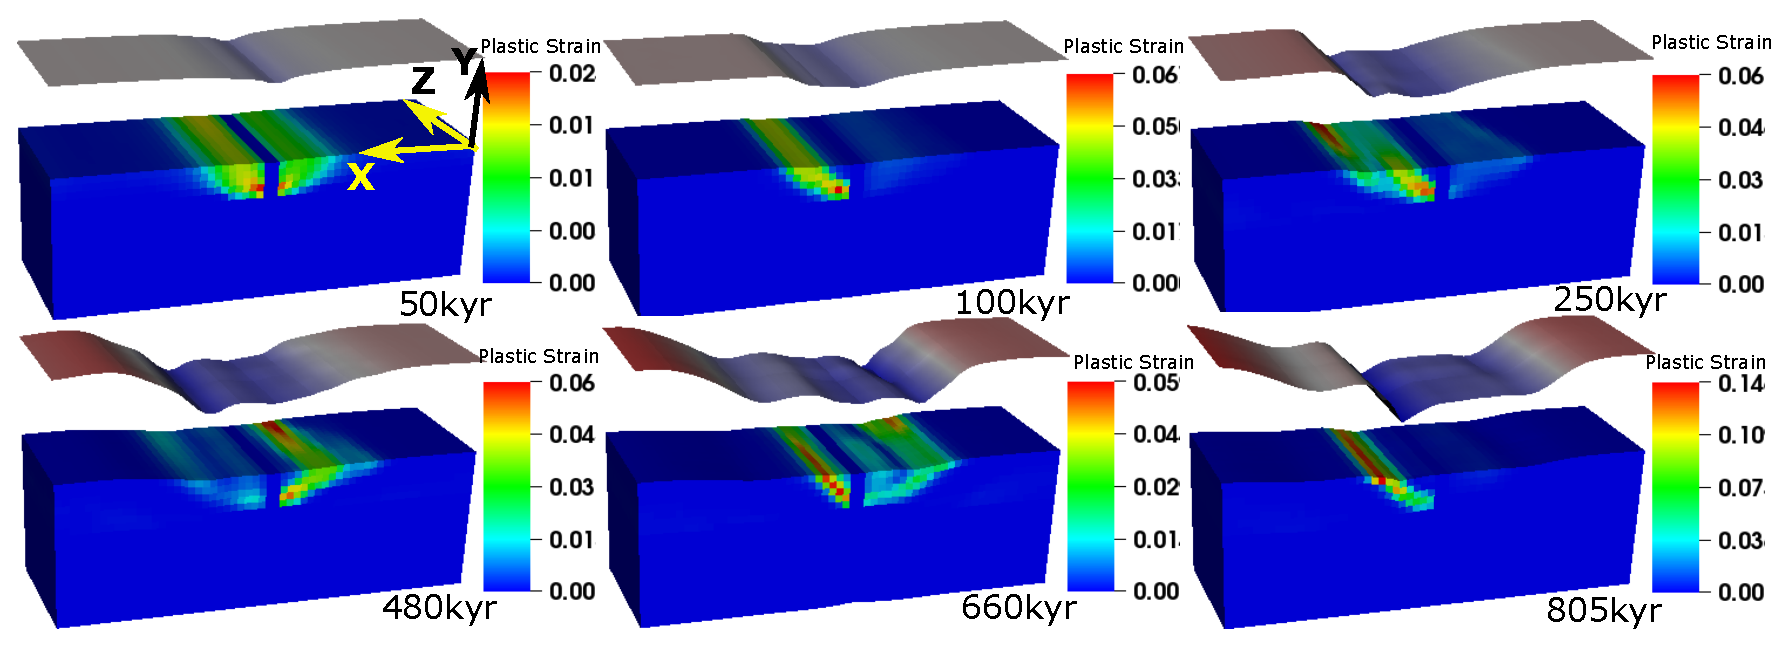
\includegraphics[width=1.0\textwidth]{./Figures/fig_Results1_3.eps}
  \caption{M88ConT2 (Table~\hyperref[Tab1_1]{\ref{Tab1_1}}). Reference model two: constant M$=0.8$ along the ridge-axis (i.e. Z axis). Type two weakening.}
 \label{fig_Results1_3}
\end{figure}   

Another reference model is the model with constant M$=0.8$ along the ridge axis as a comparison to the changing M models.

As shown in Figure~\hyperref[fig_Results1_3]{\ref{fig_Results1_3}}, this constant M along the ridge-axis model creates a median valley of $\sim 20km$ in width and $1\sim2km$ in depth which is similar to generally observation of Mid-Atlantic Ridges. The width and depth of the median valley is almost constant along the ridge-axis. The variation along the ridge-axis in breakaway and termination as well as the existence of corrugation mentioned in reference model one are not observed. 


\subsection{Effects of the functional forms of M variation}
As shown in the \annote[EC]{tables}{which table? Specify.}, \add[EC]{the models with} \annote[EC]{M28}{Before starting to use this notation, define and explain it first!} with Type one weakening is \annote[EC]{the only M range that has three functional forms data points available}{This sentence gives an impression that you didn't want to use these three but had no choice but to. This is not the case, I belive. Probably you'd want to point out that one of these three is the reference model that has been fully described earlier. So, we are in a better position to compare it with similar models with different functional forms. In fact, I think this introductory sentence can be thrown out.} 

\change[EC]{There are two phenomena that show distinct differences with respect to different functional forms.}{By comparing M28LinT1 with M28SinT1 and M28sqrtT1, I identified two main characteristics in the different behaviors of these models due to different functional forms of M variation.} One is the geometry and timing of the secondary fault. The other is the ``Cut back'' behavior. \annote[EC]{mostly observed in the square root model.}{No need to spill the beans.}

\begin{figure}[h]
  \centering
    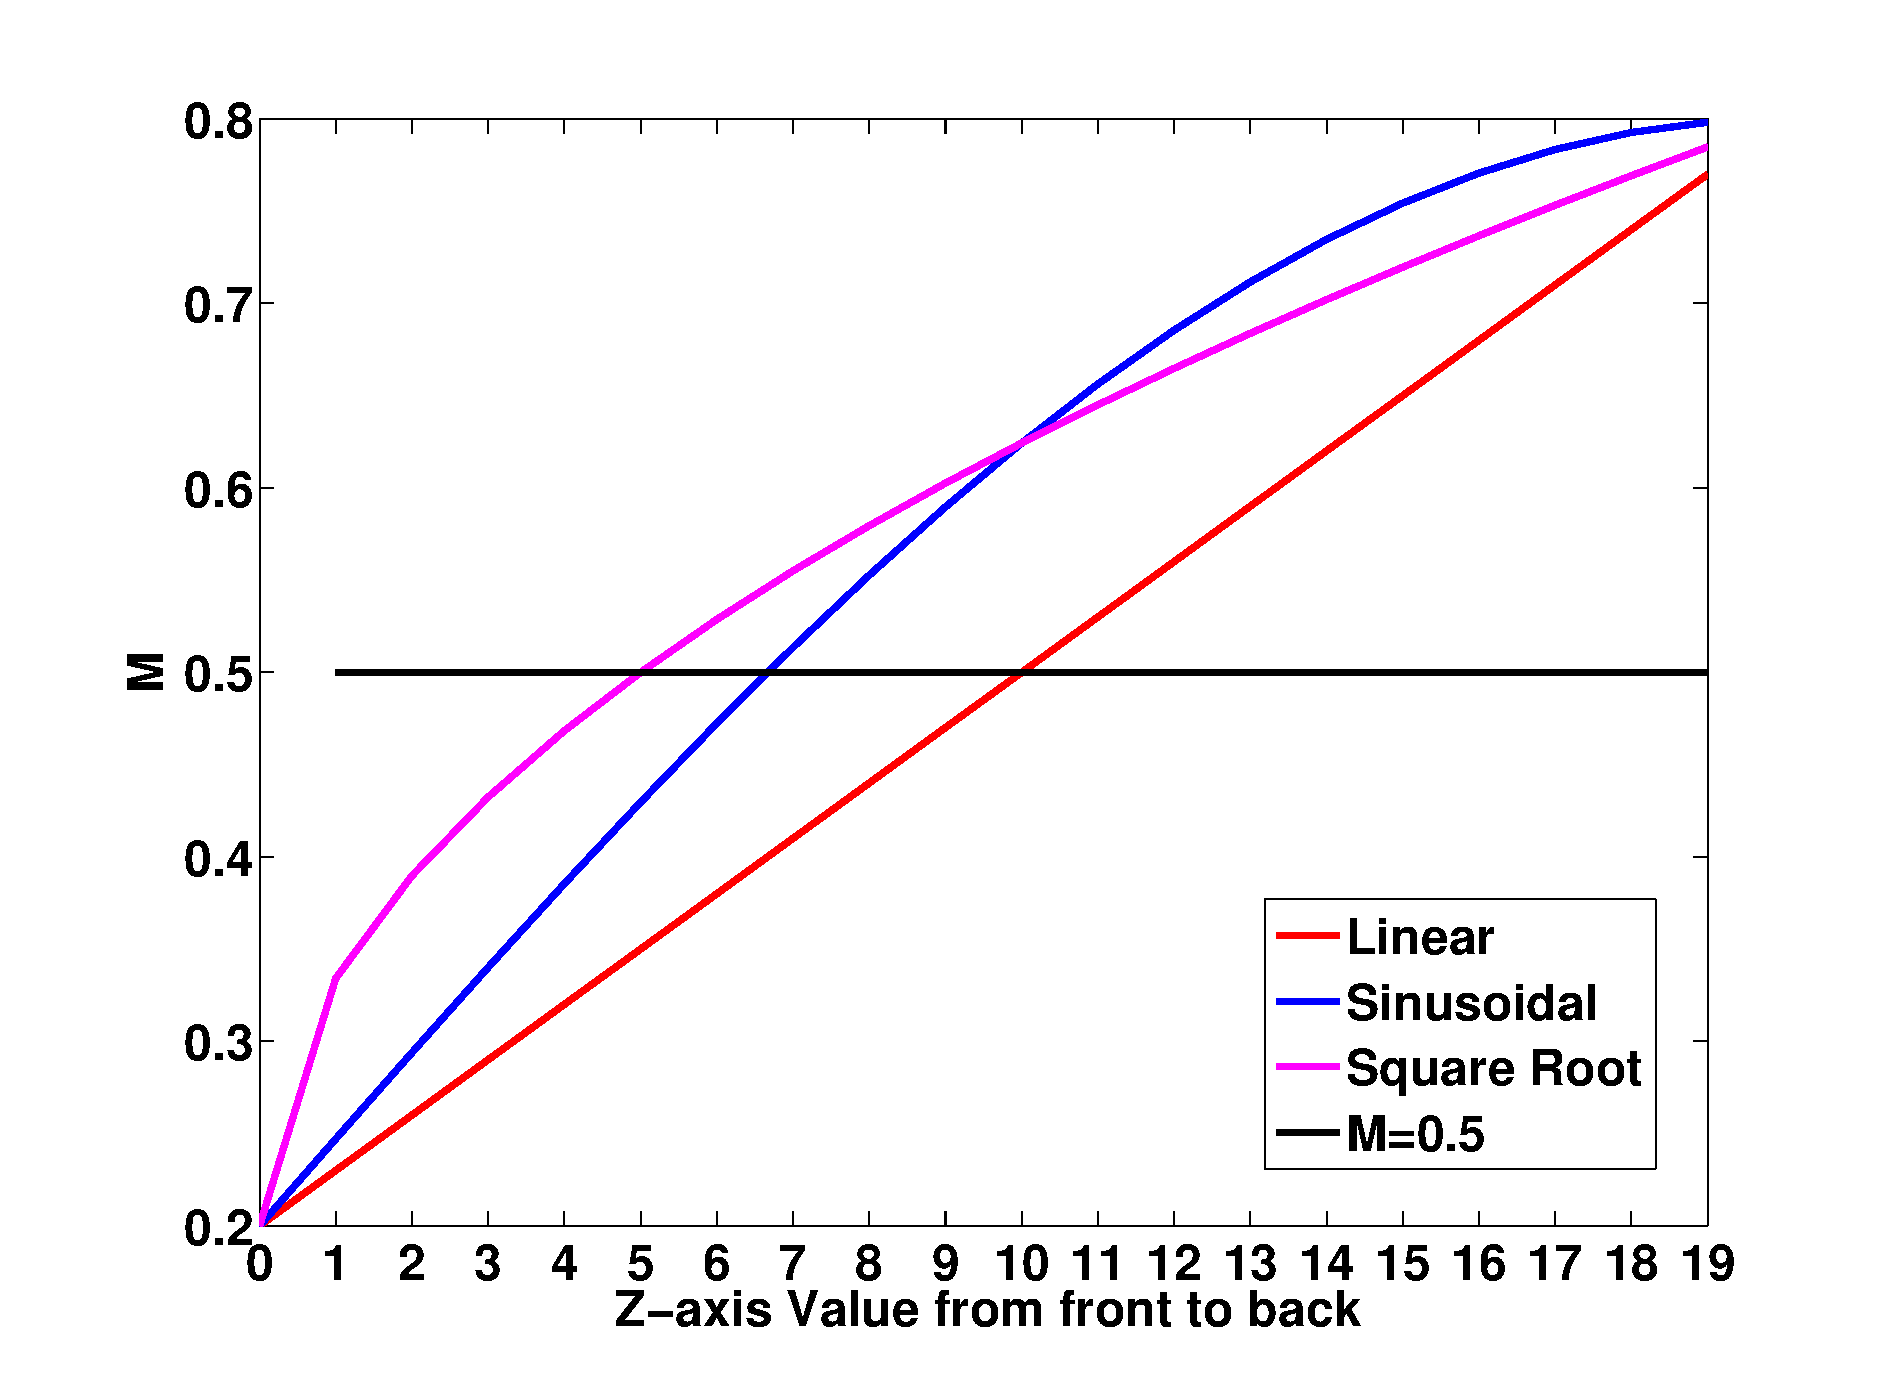
\includegraphics[width=0.6\textwidth]{./Figures/fig_Results3_1.eps}
  \caption{Three functional forms of M variation comparison. They begin to exceed the M$=0.5$ black line at Z=10, 7, 5 for linear, sinusoidal and square root respectively.}
 \label{fig_Results3_1}
\end{figure}   

\paragraph{Second Fault}\label{para_SecondaryFault}

For the linear functional form, the second fault \note[XT]{add a definition of secondary fault in the begining, here add a link of figure about primary and sec fault, enlarge the second fault and add label in the figure and use it here } at the high M side has started accommodating most of the extension at around 900kyrs and the initial detachment becomes inactive \note[XT]{(Figure~\hyperref[fig_Results4_2]{\ref{fig_Results4_2}})}{refer to Figure 8.f is better}. It nucleates from the ridge center where M$=0.5$ and then propagates to the M$=0.8$ end. %(Figure~\hyperref[fig_Results3_1]{\ref{fig_Results3_1}} where the red line begin to exceeds 0.5 at Z$=10$).
 %This secondary fault creates another dome with initial composition likely to be volcanic rather than ultramafic, however, as it evolves, if it can last long enough to cut through the whole crust, mantle materials might exhume to the surface. The composition of the domes observed at Kane magamullions is similar to this mechanism between ultramafic babel dome and eastern to it the crustal inside-corner high.  its spatial distribution is at M$>0.5$ region.

\begin{figure}[h]
  \centering
    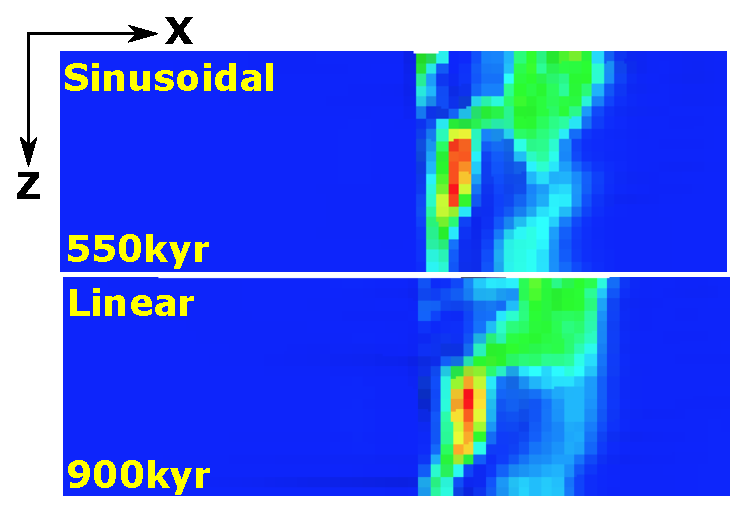
\includegraphics[width=0.6\textwidth]{./Figures/fig_Results4_2_secondary_fault_length_comparison.eps}
  \caption{M28LinT1 versus M28SinT1 (Table~\hyperref[Tab1_1]{\ref{Tab1_1}}). Secondary fault length comparison between linear and sinusoidal. Around 13 elements in length for sinusoidal compared to 11 elements for linear.}
 \label{fig_Results4_2}
\end{figure}   

For the sinusoidal form, the second fault begins to form at a much earlier time around 550kyrs (Figure~\hyperref[fig_Results4_2]{\ref{fig_Results4_2}}). The sinusoidal form consistently has higher M values than the linear form (Fig. 10), implying a greater amount of magma supply. %The total force to push the hanging wall of the detachment away from the dike is greater than that of linear. The larger the force,
The first forming fault moves away from the ridge axis faster and locks earlier in the case of the sinusoidal form. As a result, the second fault appears earlier than in the case of the linear M variation. In addition, the sinusoidal form produces the second fault with a greater along-strike dimension than the linear form because this length is proportional to the length of the M $\ge$ 0.5 portion of the ridge (Figure~\hyperref[fig_Results3_1]{\ref{fig_Results3_1}}). 
For square root, there is no secondary fault forming because the ``cut back'' behavior releases the tensional stress in the hanging wall.

\paragraph{Cut-back}\label{para_CutBack}

\begin{figure}[h]
  \centering
    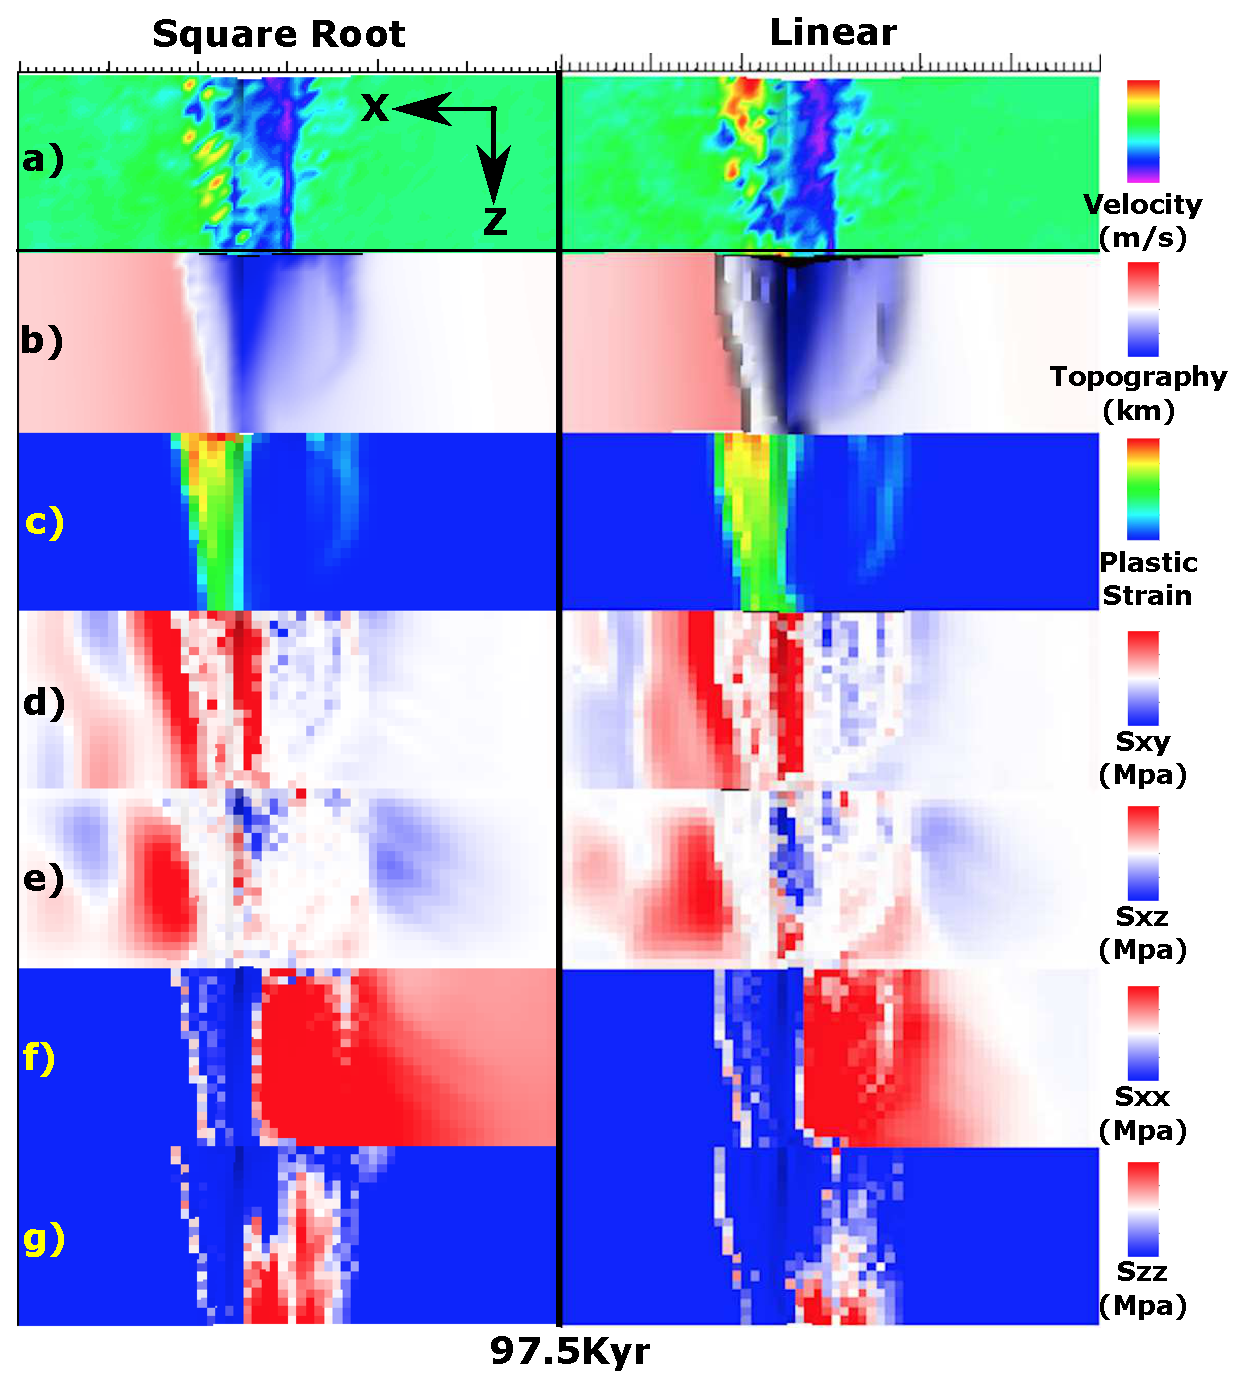
\includegraphics[width=0.6\textwidth]{./Figures/fig_Results4_3_sqrt_vs_lin_cut_back_97kyr.eps}
  \caption{M28LinT1 versus M28SqrtT1 (Table~\hyperref[Tab1_1]{\ref{Tab1_1}}) at 97kyr. View from top of the model.}
 \label{fig_Results4_3_1}
\end{figure}  

\begin{figure}[h]
  \centering
    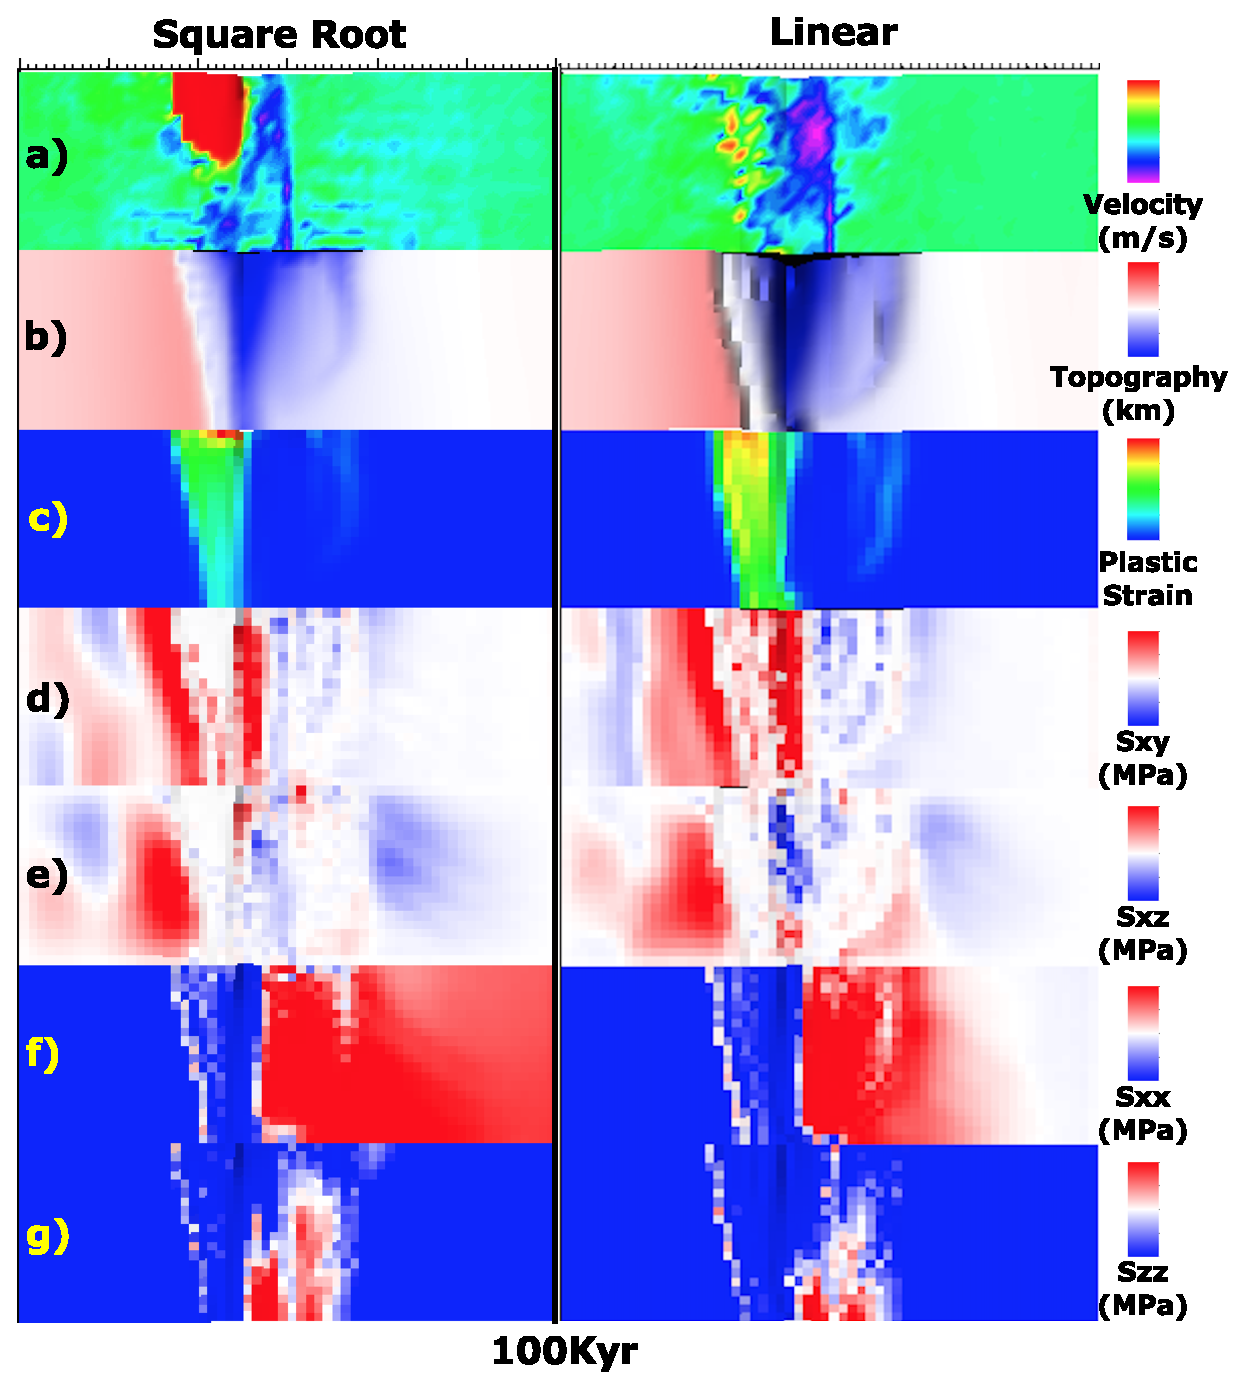
\includegraphics[width=0.6\textwidth]{./Figures/fig_Results4_3_sqrt_vs_lin_cut_back_100kyr.eps}
  \caption{M28LinT1 versus M28SqrtT1 (Table~\hyperref[Tab1_1]{\ref{Tab1_1}}) at 100kyr. View from top of the model.}
 \label{fig_Results4_3_2}
\end{figure} 

\note[XT]{Define a cut-back and think about a different name.}
The cut-back characterizes but are not limited to the models with the square root form of M variation.\note[XT]{exclusively about the square root models?} As shown in Figure~\hyperref[fig_Results4_3_1]{\ref{fig_Results4_3_1}}, Figure~\hyperref[fig_Results4_3_1]{\ref{fig_Results4_3_2}} and Figure~\hyperref[fig_Results4_4]{\ref{fig_Results4_4}} \note[XT]{Bring up Fig. 26 here and incude only the cut-back panel.}, between 97.5kyr and 100kyr, there are cut-backs in the square root model M28SqrtT1 at the low M side where hanging walls with surface area of $\sim$ 60 km$^{2}$ and $\sim$ 120 km$^{2}$ (the red block) suddenly rebound backwards towards the ridge-axis as seen in 100kyr and 160kyr (Figure~\hyperref[fig_Results4_3_1]{\ref{fig_Results4_3_2}.a} and Figure~\hyperref[fig_Results4_4]{\ref{fig_Results4_4}.d,e,f}), along with sudden topography drop (Figure~\hyperref[fig_Results4_4]{\ref{fig_Results4_4}.d,e} 2nd row), $\sigma_{xy}$ and $\sigma_{xz}$ released, termination falls back (Figure~\hyperref[fig_Results4_4]{\ref{fig_Results4_4}.f} 3rd row). 

\subsection{Effects of the weakening rate}

According to our available twelve 3D models, we have three pairs of models that both have Type one and Type two \note[XT]{might want to add a ref to the section defining these.} weakening while the range of M and functional form are maintained to be the same. They are M57SinT1/T2, M58SinT1/T2 and M58SqrtT1/T2.

\paragraph{M57SinT1 versus M57SinT2}

\begin{figure}[h]
 \centering
  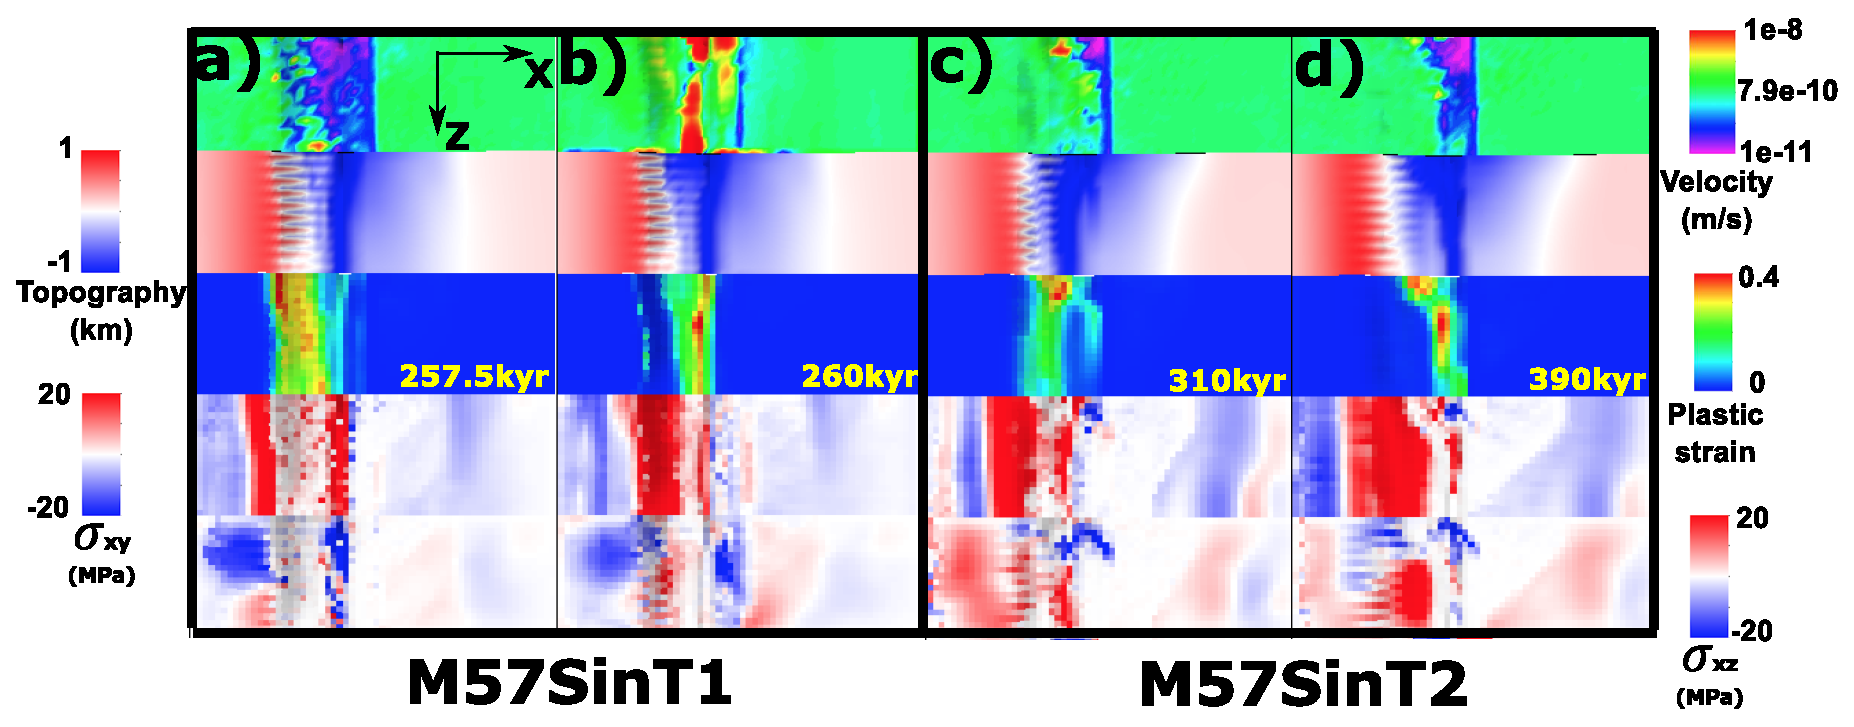
\includegraphics[width=1.0\textwidth]{./Figures/fig_Results_Weakening_2_M57SinT1VST2_CutbackVSsecondaryFault.eps}
 \caption{M57SinT2 versus M57SinT1 (Table~\hyperref[Tab1_1]{\ref{Tab1_1}}). a) and b) are for M57SinT2, c) and d) are for M57SinT1.}
\label{fig_Results_Weakenging_2}
\end{figure}

Initially, both models develop normal faults on both sides of the ridge axis\note[XT]{no hyphen in ``ridge axis''.} at the low M side. In the model with the faster weakening rate (M57SinT1), faults propagate toward the high M side and cut through the whole crust by 25kyr but this process completes later at 50 kyr in the model with the slower weakening rate (M57SinT2). At around 310kyr, the second fault appears at the high M side\note[XT]{instead of z=5, use a M value.} of M57SinT2 while where M $<=$\annote[XT]{5}{some M value}, the initial fault remains active (Figure~\hyperref[fig_Results_Weakenging_2]{\ref{fig_Results_Weakenging_2}.a) and b)}). However, when the weakening is fast (M57SinT1), cut-back happens at around 260kyr and help to maintain a high angle fault with closer to ridge-axis termination. The initial fault remains, no secondary fault forming (Figure~\hyperref[fig_Results_Weakenging_2]{\ref{fig_Results_Weakenging_2}.a) and b)}). In addition, the width of median valley at low M side is wider for M57SinT2 than M57SinT1 (Figure~\hyperref[fig_Results_Weakenging_2]{\ref{fig_Results_Weakenging_2}.a) and b) versus c) and d)}) due to slower weakening (Type two) alows a more distributed tensional stress $\sigma_{xx}$ rather than fast weakening that once a fault is established, larger amount of tensional stress $\sigma_{xx}$ will be released at the fault.  

\begin{figure}[h]
 \centering
  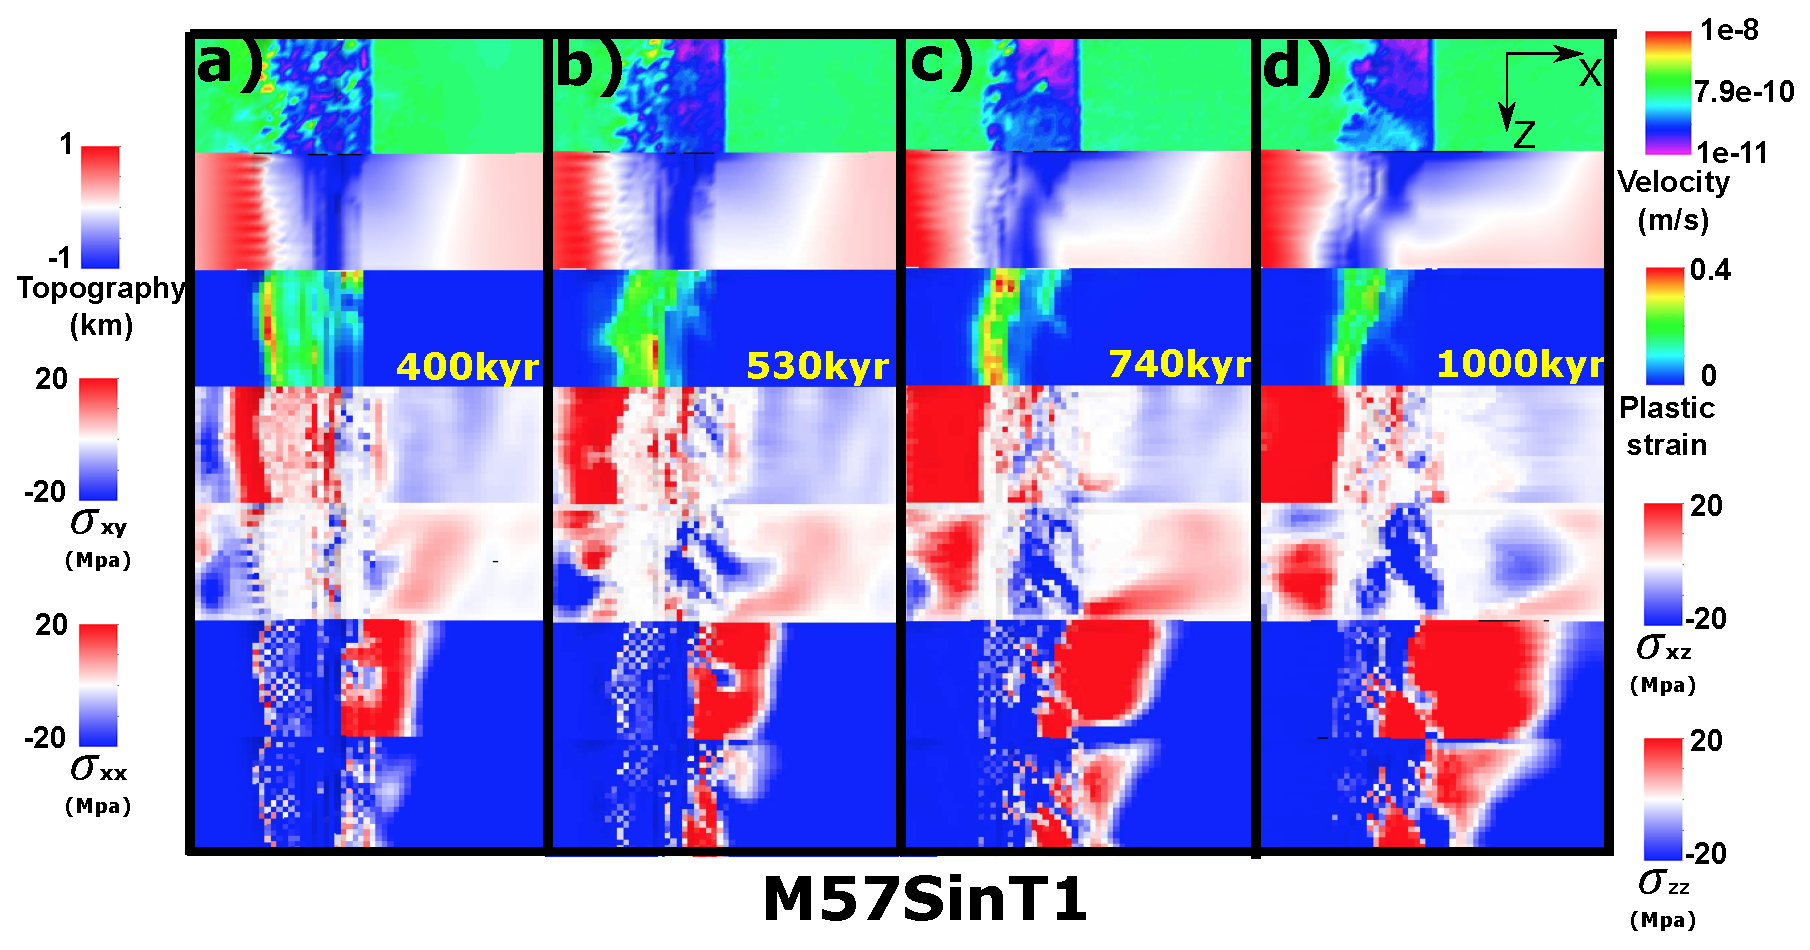
\includegraphics[width=1.0\textwidth]{./Figures/fig_Results_Weakening_3_M57SinT1_time_evolution.eps}
 \caption{M57SinT1 (Table~\hyperref[Tab1_1]{\ref{Tab1_1}}) faulting and stress evolution with respect to time.}
\label{fig_Results_Weakenging_3}
\end{figure}

\paragraph{M57SinT1}\label{para_M57SinT1}

For M57SinT1, as shown in Figure~\hyperref[fig_Results_Weakenging_3]{\ref{fig_Results_Weakenging_3}}, at 400kyr (Figure~\hyperref[fig_Results_Weakenging_3]{\ref{fig_Results_Weakenging_3}.a}), there is a antithetic fault forming at the low M side accommodating part of the extension, which results in a curved termination at the far frontier. As it evolve (530kyr (Figure~\hyperref[fig_Results_Weakenging_3]{\ref{fig_Results_Weakenging_3}.b})), the termination at the low M side further recedes backward while the termination at the center (Z$=11\sim13$) extends further. This curved termination leads to a curved topography (white curve in the second row). As the fault evolves and bends further away from the axis, at the time of 740kyr, another antithetic fault forming again at the low M side (Figure~\hyperref[fig_Results_Weakenging_3]{\ref{fig_Results_Weakenging_3}.c}). It doesn't take the place of initial fault and disapear soon, however, it again releases tensional stress and results in that the termination at far front recedes backward. At 1000kyr (Figure~\hyperref[fig_Results_Weakenging_3]{\ref{fig_Results_Weakenging_3}.d}), an Atlantiss Massif shape OCC is produced (low M side (lower magma supply) has a wider dome and high M side (higher magma supply) has a narrower dome) due to the along ridge-axis termination evolution. Corrugations with wavelength varying from hundreds to kilometers are also created.       

\begin{figure}[h]
 \centering
  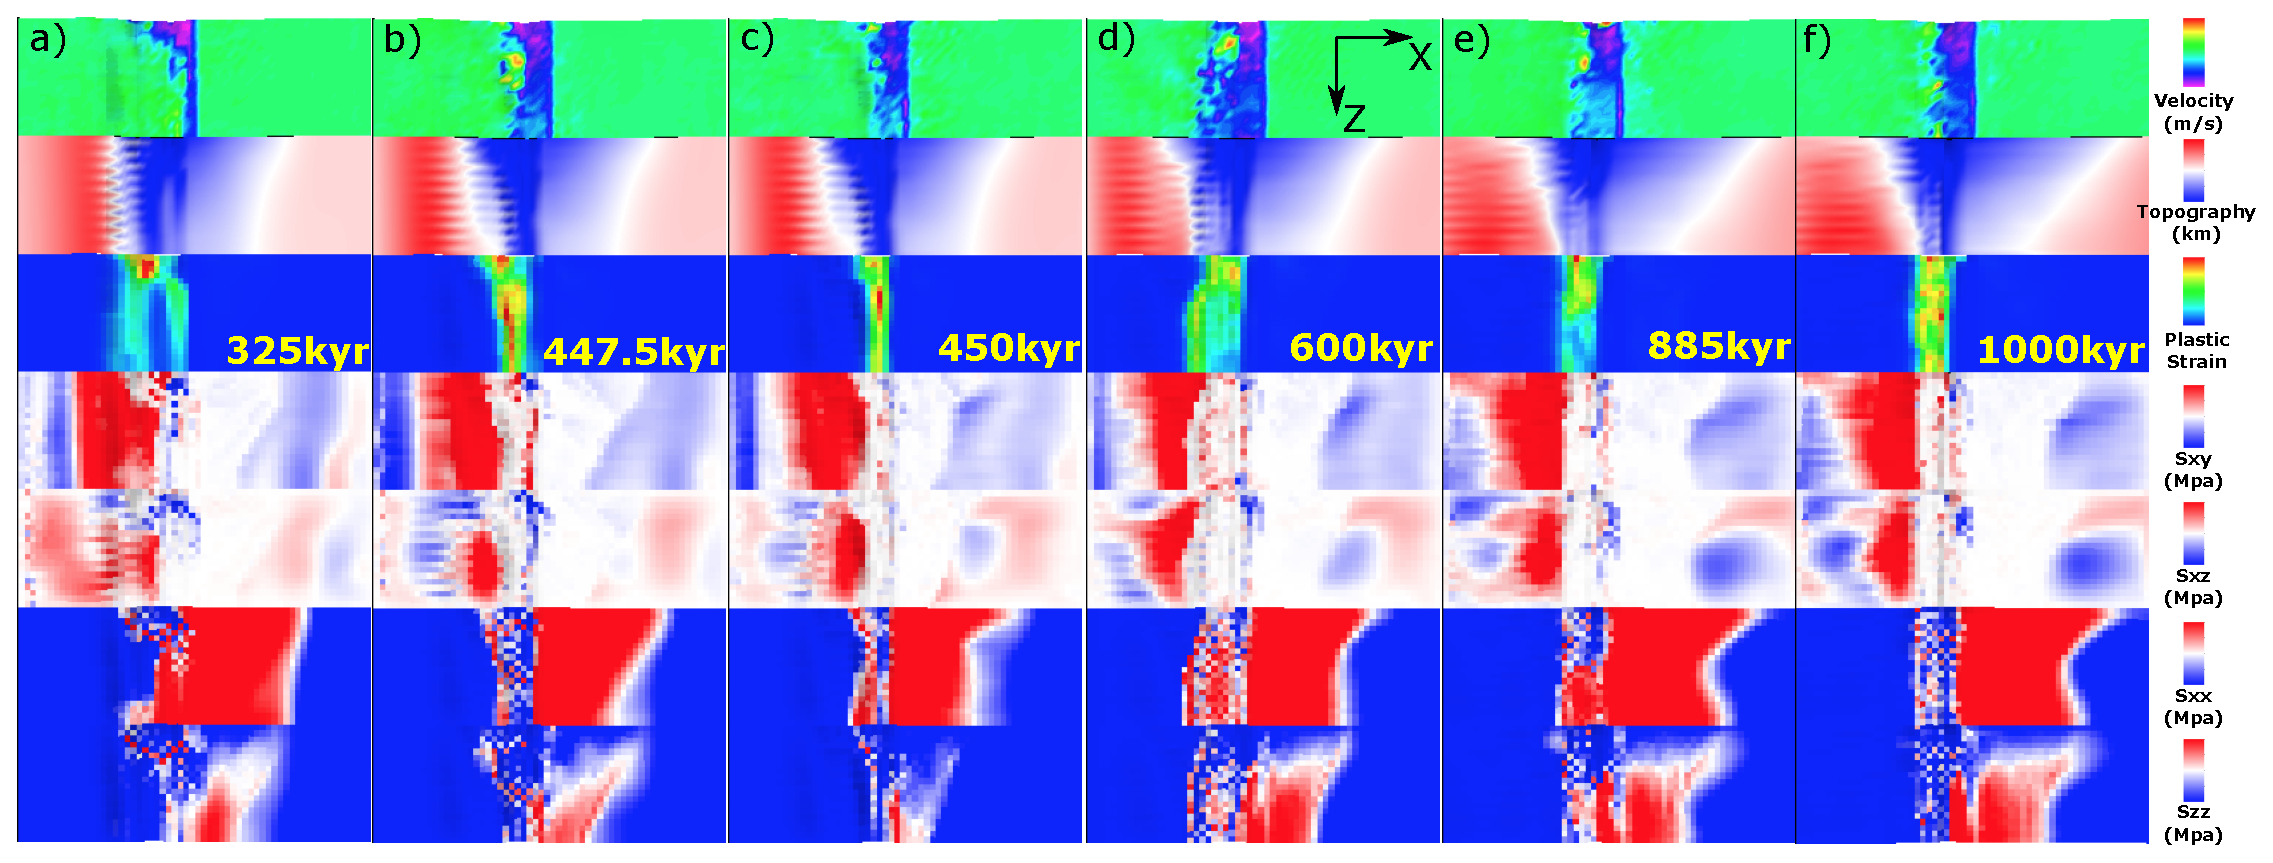
\includegraphics[width=1.0\textwidth]{./Figures/fig_Results_Weakening_4_M57SinT2_time_evolution.eps}
 \caption{M57SinT2 (Table~\hyperref[Tab1_1]{\ref{Tab1_1}}) faulting and stress evolution with respect to time.}
\label{fig_Results_Weakenging_4}
\end{figure}

\paragraph{M57SinT2}\label{para_M57SinT2}

For M57SinT2, as shown in Figure~\hyperref[fig_Results_Weakenging_4]{\ref{fig_Results_Weakenging_4}}, instead of maintaining one fault all the time for M57SinT1, it creats secondary fault at high M side with different mechanism several times. A secondary fault is created at 325kyr (Figure~\hyperref[fig_Results_Weakenging_4]{\ref{fig_Results_Weakenging_4}.a}), when a new near axis normal fault take the place of the initial one at high M side. Between 447.5kyr (Figure~\hyperref[fig_Results_Weakenging_4]{\ref{fig_Results_Weakenging_4}.b}) and 450kyr (Figure~\hyperref[fig_Results_Weakenging_4]{\ref{fig_Results_Weakenging_4}.c}), termination falls back, and as it evolve, termination at the high M side extends further at 600kyr (Figure~\hyperref[fig_Results_Weakenging_4]{\ref{fig_Results_Weakenging_4}.d}). At 885kyr (Figure~\hyperref[fig_Results_Weakenging_4]{\ref{fig_Results_Weakenging_4}.e}), a secondary fault propagates from low Z to high Z and terminates the further extended fault at high Z and maintain a near ridge-axis termination.

\subsubsection{M58SinT1 versus M58SinT2}

A major difference between M58SinT1 and M58SinT2 is that M58SinT1 keep faulting at one side of the ridge-axis while M58SinT2's fault alternates.

\begin{figure}[h]
 \centering
  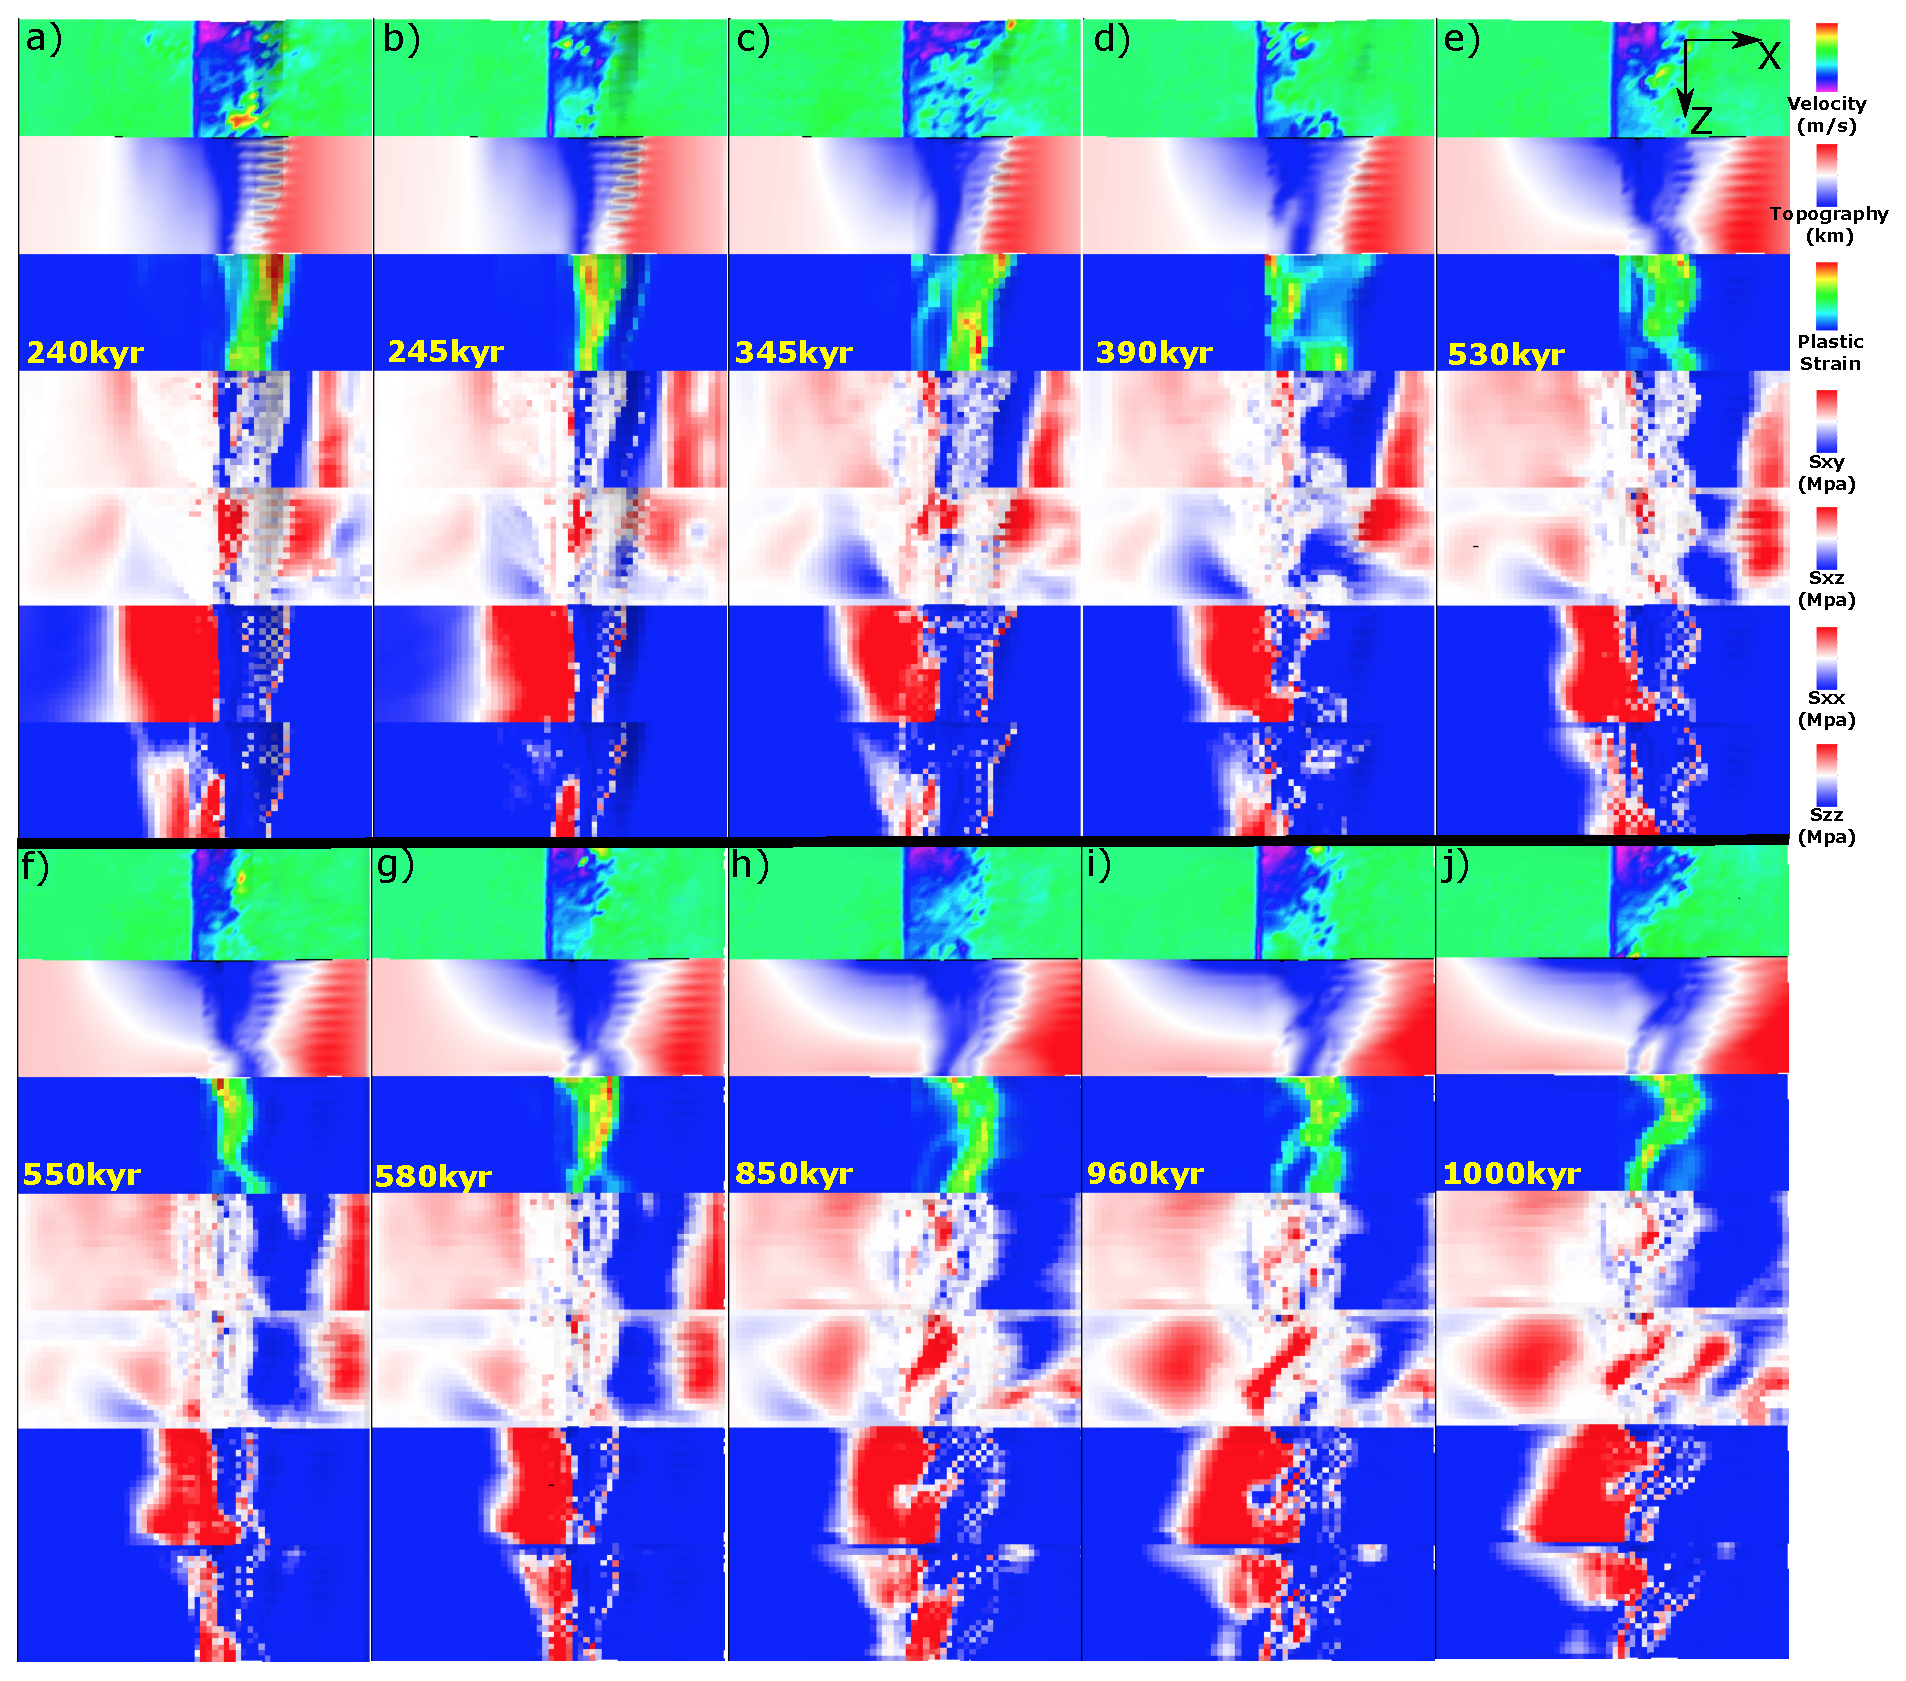
\includegraphics[width=1.0\textwidth]{./Figures/fig_Results_Weakening_5_M58SinT1_time_evolution.eps}
 \caption{M58SinT1 (Table~\hyperref[Tab1_1]{\ref{Tab1_1}}) faulting and stress evolution with respect to time.}
\label{fig_Results_Weakenging_5}
\end{figure}

\paragraph{M58SinT1}\label{para_M58SinT1}

As shown in Figure~\hyperref[fig_Results_Weakenging_5]{\ref{fig_Results_Weakenging_5}}, in 1Myr, the fault keeps on the right hand side of the ridge-axis. It evolves dynamically. Between 240kyr (Figure~\hyperref[fig_Results_Weakenging_5]{\ref{fig_Results_Weakenging_5}.a}) and 245kyr (Figure~\hyperref[fig_Results_Weakenging_5]{\ref{fig_Results_Weakenging_5}.b}), there is a cut back. At 345kyr (Figure~\hyperref[fig_Results_Weakenging_5]{\ref{fig_Results_Weakenging_5}.c}), at low Z side, there are two offsetted antithetic faults (Z=$1\sim2$ and Z=$5\sim9$) in the hanging wall begin to evolve and soon connect to each other forming anastomosing fault zone. At 390kyr (Figure~\hyperref[fig_Results_Weakenging_5]{\ref{fig_Results_Weakenging_5}.d}), the new near axis anastomosing fault zone replace the old further away from ridge-axis detachment. There is dextral $\sigma_{xz}$ forming on the right hand side of the new anastomosing fault zone ((Figure~\hyperref[fig_Results_Weakenging_5]{\ref{fig_Results_Weakenging_5}.d}), row 5) due to the offset between the new near axis fault at low Z side and extended further fault at high Z side and leads to the development of a $\sim45\degree$ shear zone connection between the new near axis fault zone at low Z side and the further away from axis original detachment at high Z side. It also creates a curved termination which will lead to a curved topography (boundary between blue and white) seen at 530kyr (Figure~\hyperref[fig_Results_Weakenging_5]{\ref{fig_Results_Weakenging_5}.e}). Note that this curved termination can be a mechanism for producing large wavelength (several kilometers) undulating corrugations. Between 530kyr (Figure~\hyperref[fig_Results_Weakenging_5]{\ref{fig_Results_Weakenging_5}.e}) and 550kyr (Figure~\hyperref[fig_Results_Weakenging_5]{\ref{fig_Results_Weakenging_5}.f}), there is another cut back happens. Terminations fall backwards to near ridge-axis position. At 580kyr (Figure~\hyperref[fig_Results_Weakenging_5]{\ref{fig_Results_Weakenging_5}.g}), at the high Z side, a new near rigde-axis high angle normal fault begin to initiate under the assistance of rotational force from low Z side due to along ridge-axis coupling. This produces a large rider block with several kilometers in its length scale. Previous ``S'' curved termination now evolves to a half circle curve and it soon affects the curve of topography as seen at 850kyr (Figure~\hyperref[fig_Results_Weakenging_5]{\ref{fig_Results_Weakenging_5}.h}). Due to along ridge-axis variation in diking, a large sinistral shear zone (red region $\sim40\degree$ oblique to ridge axis seen in 5th row of 960kyr (Figure~\hyperref[fig_Results_Weakenging_5]{\ref{fig_Results_Weakenging_5}.i})) keep developing and cut the circle curved fault zone at 850kyr (Figure~\hyperref[fig_Results_Weakenging_5]{\ref{fig_Results_Weakenging_5}.h}) into a new fault zone with higher curvature as seen in 1000kyr (Figure~\hyperref[fig_Results_Weakenging_5]{\ref{fig_Results_Weakenging_5}.j}).         

\begin{figure}[h]
 \centering
  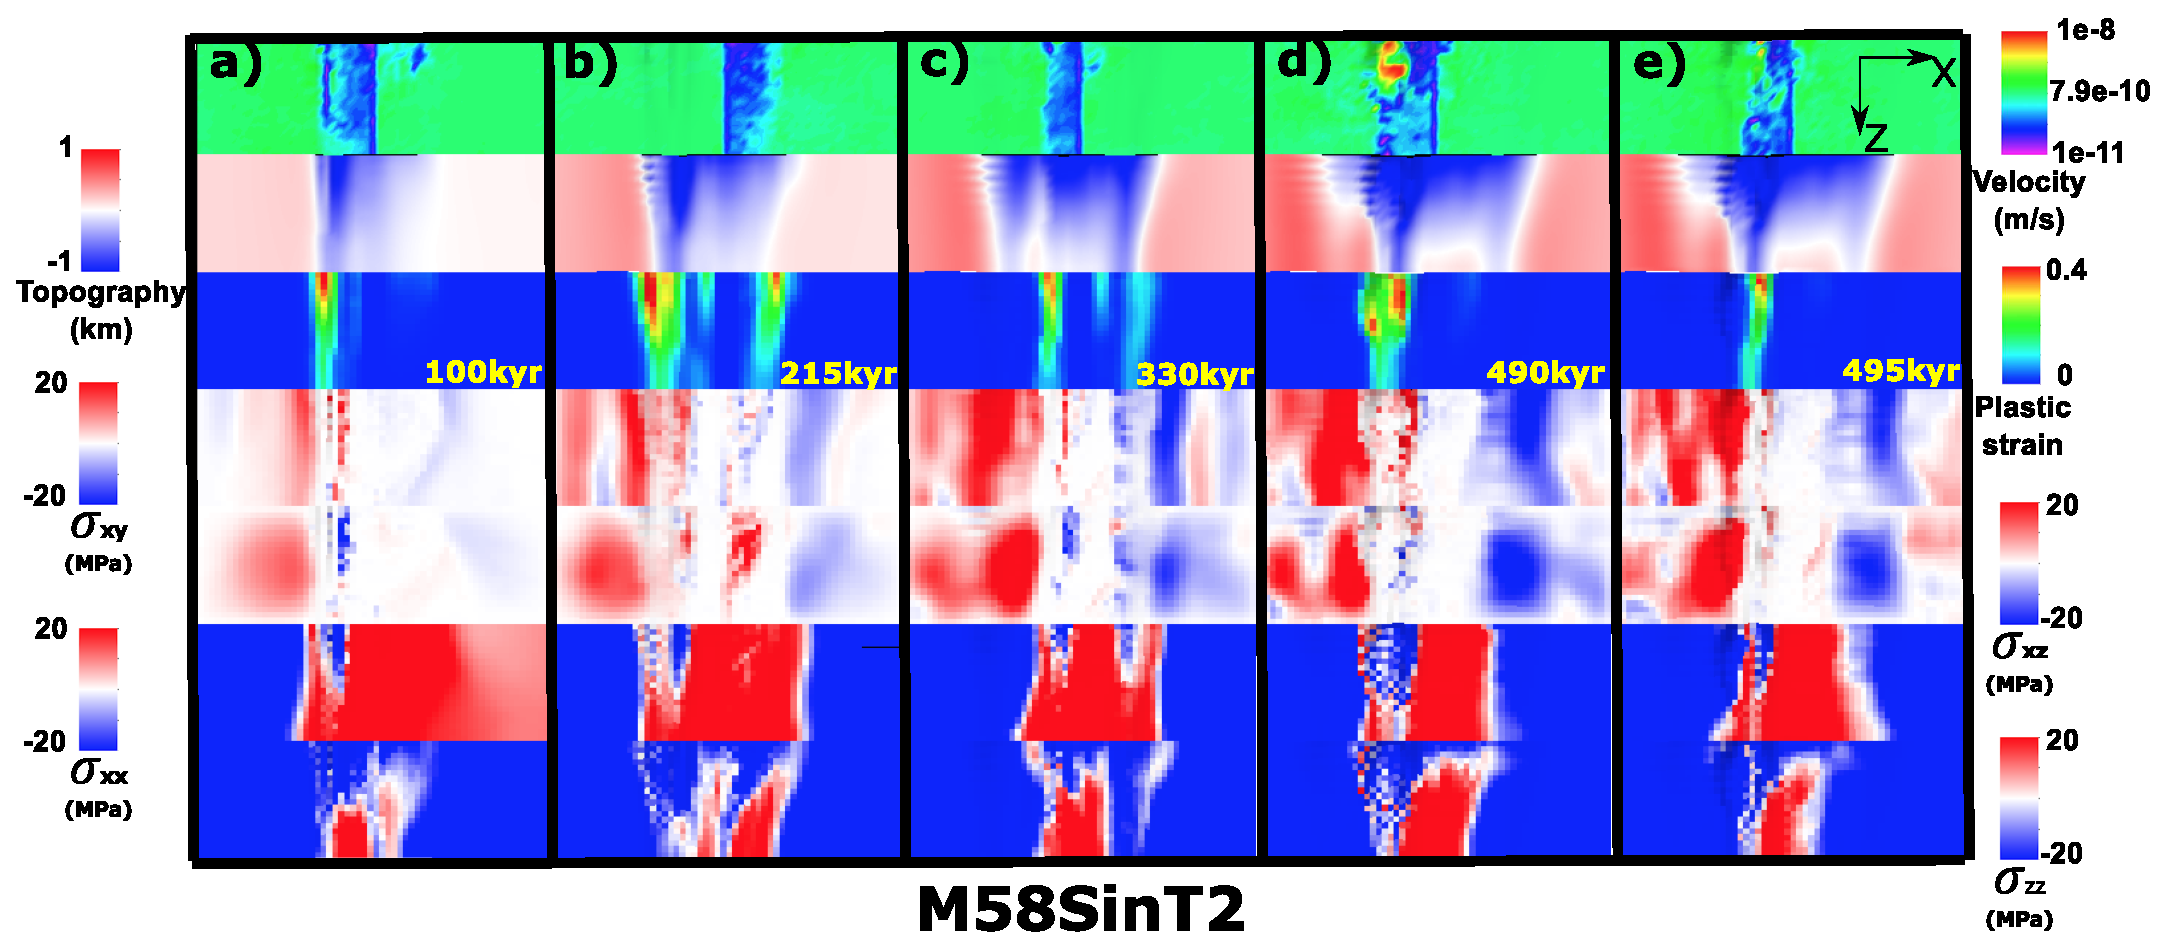
\includegraphics[width=1.0\textwidth]{./Figures/fig_Results_Weakening_6_M58SinT2_time_evolution.eps}
 \caption{M58SinT2 (Table~\hyperref[Tab1_1]{\ref{Tab1_1}}) faulting and stress evolution with respect to time.}
\label{fig_Results_Weakenging_6}
\end{figure}

\paragraph{M58SinT2}\label{para_M58SinT2}

As shown in Figure~\hyperref[fig_Results_Weakenging_6]{\ref{fig_Results_Weakenging_6}}, the fault initiates on the left hand side of the ridge-axis (Figure~\hyperref[fig_Results_Weakenging_6]{\ref{fig_Results_Weakenging_6}.a}). Low Z side extends further than high Z side. It takes around 100kyr to form into a localized fault plane due to slower rate of weakening. At 215kyr (Figure~\hyperref[fig_Results_Weakenging_6]{\ref{fig_Results_Weakenging_6}.b}), another fault on the conjugate plate begin to evolve and replaces the initial one. As seen from (Figure~\hyperref[fig_Results_Weakenging_6]{\ref{fig_Results_Weakenging_6}.b}), corrugations are created at low Z side. At 330kyr, a third fault forming at the left hand side of the ridge-axis. Between 490kyr (Figure~\hyperref[fig_Results_Weakenging_6]{\ref{fig_Results_Weakenging_6}.d}) and 495kyr (Figure~\hyperref[fig_Results_Weakenging_6]{\ref{fig_Results_Weakenging_6}.e}), there is a cut back.

\subsubsection{M58SqrtT1 versus M58SqrtT2}
The major difference between M58SqrtT1 and M58SqrtT2 is also whether the normal fault alternates or not.

\paragraph{M58SqrtT1}\label{para_M58SqrtT1}

As shown in Figure~\hyperref[fig_Results_Weakenging_7]{\ref{fig_Results_Weakenging_7}}, initially, there is a 5 element offset between breakaways along the ridge-axis due to along ridge-axis variation in diking (Figure~\hyperref[fig_Results_Weakenging_7]{\ref{fig_Results_Weakenging_7}.a}). At 370kyr (Figure~\hyperref[fig_Results_Weakenging_7]{\ref{fig_Results_Weakenging_7}.b}), there is a vertical tensile failure at Z$=1\sim2$. Two parallel dextral (blue) shear regions are seen (5th row). The low Z shear zone assists in the shear failure observed at 400kyr (Figure~\hyperref[fig_Results_Weakenging_7]{\ref{fig_Results_Weakenging_7}.c}), and it develops into near ridge-axis normal fault (Z=$4\sim12$) and propagates to high Z side which eventually cuts through and reaches Z$=20$ and replaces the initial extended fault at high Z side at 460kyr (Figure~\hyperref[fig_Results_Weakenging_7]{\ref{fig_Results_Weakenging_7}.d}). The vertical tensile failure zone at Z$=1\sim3$ (Figure~\hyperref[fig_Results_Weakenging_7]{\ref{fig_Results_Weakenging_7}.d} 3rd row) begin to evolve and assists in the initiation of a new near ridge-axis high angle normal fault which connect with the fault at the high Z side (Figure~\hyperref[fig_Results_Weakenging_7]{\ref{fig_Results_Weakenging_7}.e}) at 590kyr. At 660kyr (Figure~\hyperref[fig_Results_Weakenging_7]{\ref{fig_Results_Weakenging_7}.f} 3rd row), there is a hint of high angle normal faulting at Z$=1\sim3$ of conjugate plate. But it doesn't develop. At 730kyr (Figure~\hyperref[fig_Results_Weakenging_7]{\ref{fig_Results_Weakenging_7}.g} 5th row), a dextral (blue) shear zone at the low Z side help to create the faulting pattern seen at 780kyr (Figure~\hyperref[fig_Results_Weakenging_7]{\ref{fig_Results_Weakenging_7}.h} 3rd row), a concave termination with a wavelenth of 10 kilometers and it has the potential to create a large wavelength corrugation. Meanwhile, at the low Z side, near the ridge-axis, there is a antithetic fault forming at the hanging wall of the detachment and it later propagates to high Z side (Figure~\hyperref[fig_Results_Weakenging_7]{\ref{fig_Results_Weakenging_7}.i}). From 820kyr to 880kyr, the antithetic fault evolves to near ridge-axis normal fault and connects with the detachment at the high Z side (Figure~\hyperref[fig_Results_Weakenging_7]{\ref{fig_Results_Weakenging_7}.j}). In addition, a tensile failure shows its hint at the low Z side (Z$=1\sim5$) of the conjugate plate.         

\begin{figure}[h]
 \centering
  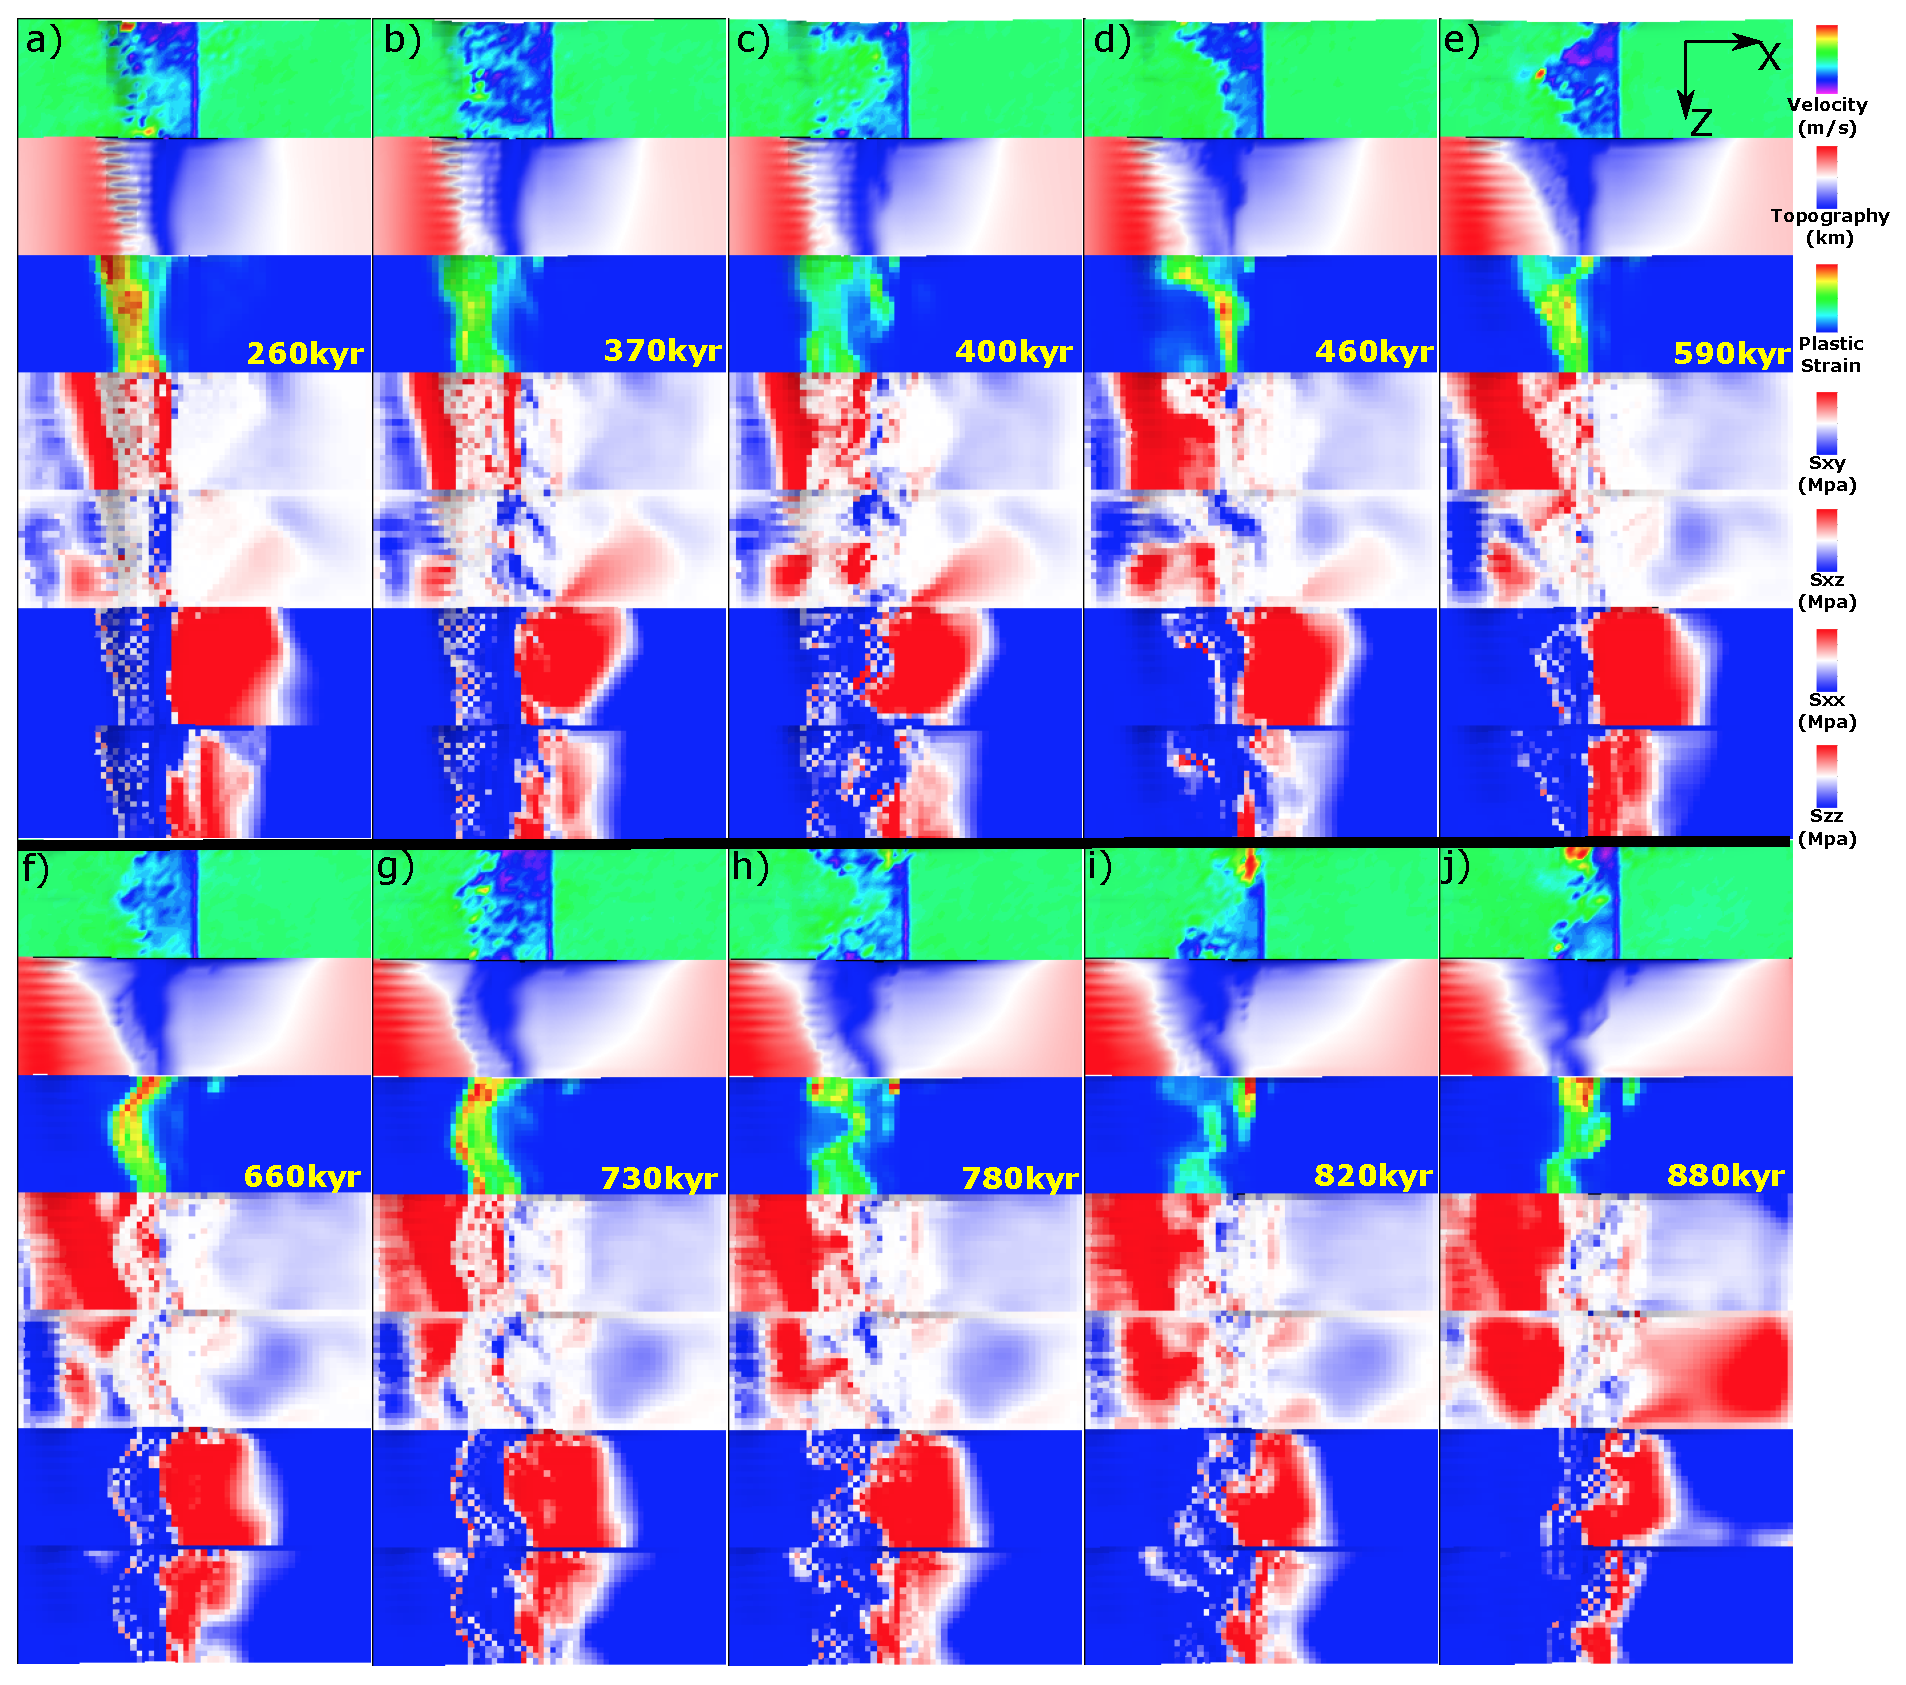
\includegraphics[width=1.0\textwidth]{./Figures/fig_Results_Weakening_7_M58SqrtT1_time_evolution.eps}
 \caption{M58SqrtT1 (Table~\hyperref[Tab1_1]{\ref{Tab1_1}}) faulting and stress evolution with respect to time.}
\label{fig_Results_Weakenging_7}
\end{figure}

\paragraph{M58SqrtT2} \label{para_M58SqrtT2}

\begin{figure}[h]
 \centering
  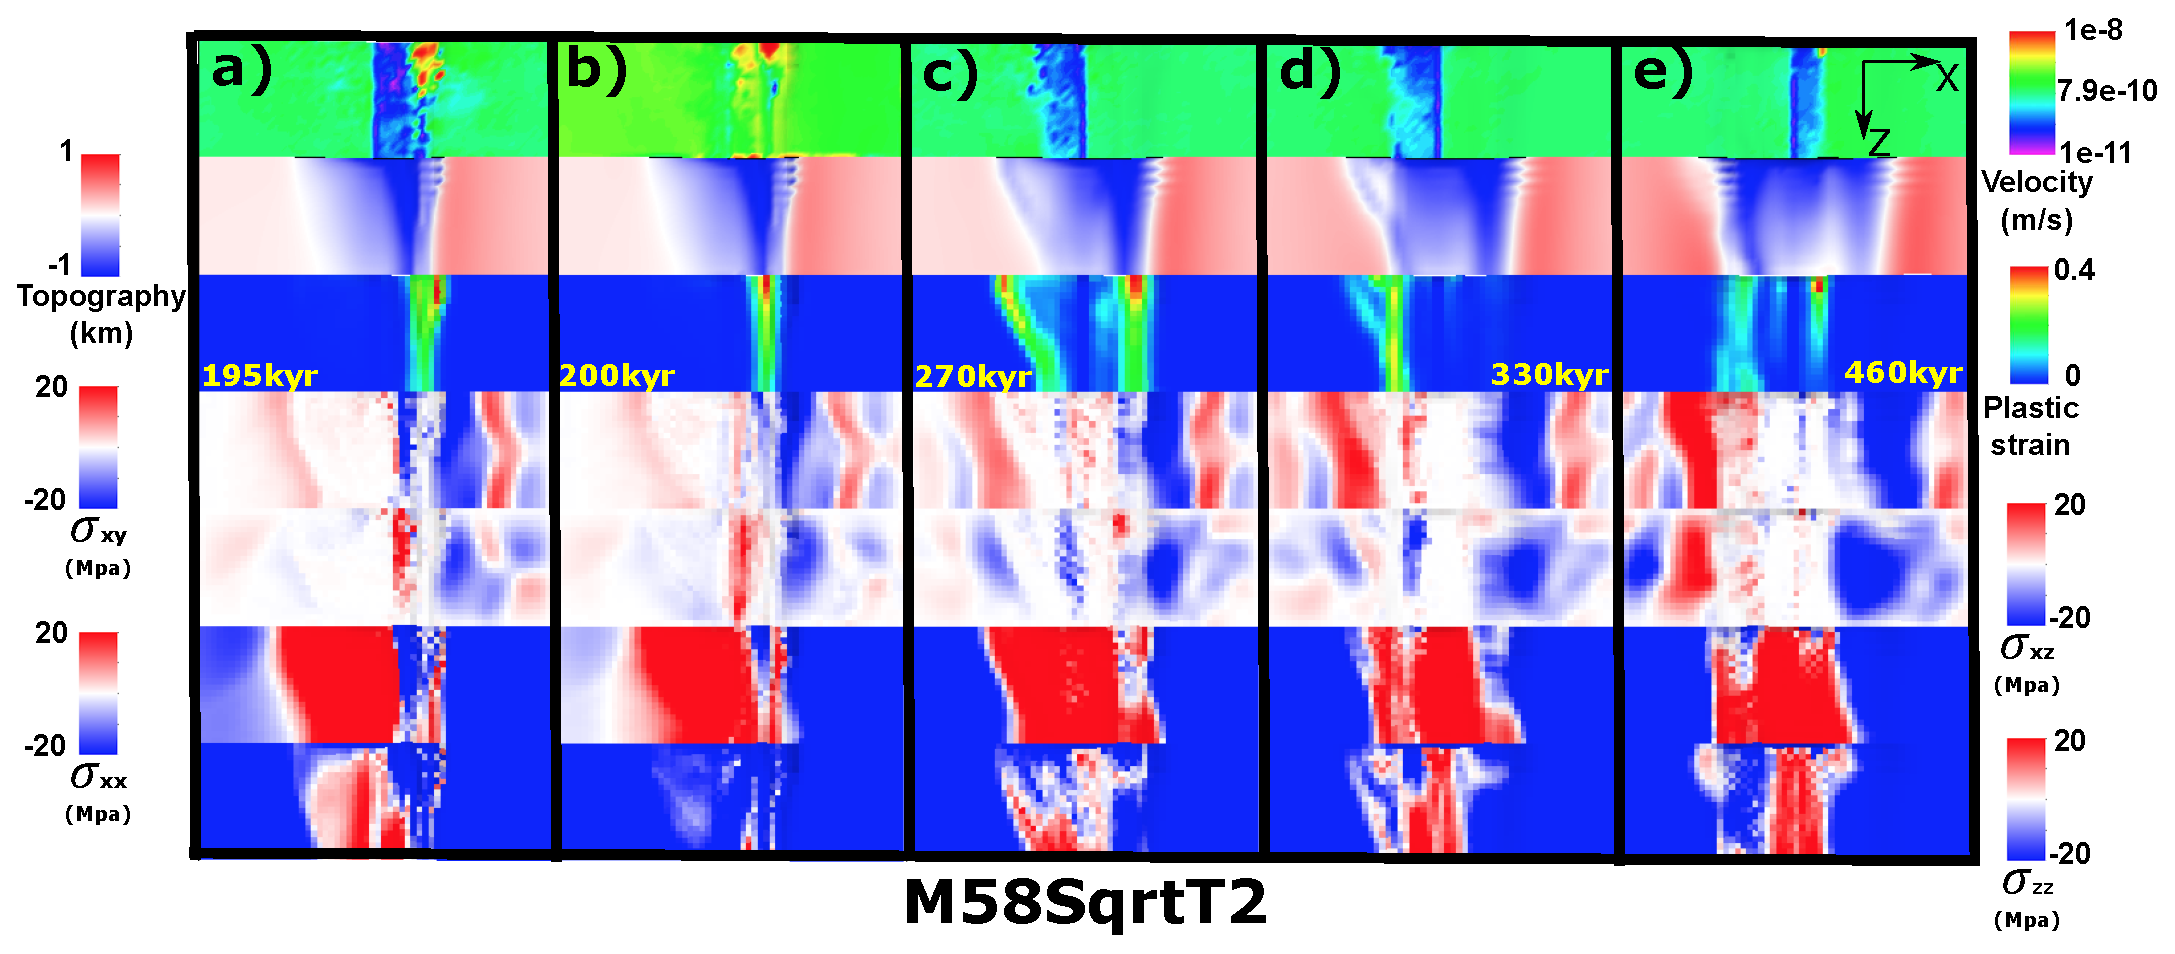
\includegraphics[width=1.0\textwidth]{./Figures/fig_Results_Weakening_8_M58SqrtT2_time_evolution.eps}
 \caption{M58SqrtT2 (Table~\hyperref[Tab1_1]{\ref{Tab1_1}}) faulting and stress evolution with respect to time.}
\label{fig_Results_Weakenging_8}
\end{figure}

As shown in Figure~\hyperref[fig_Results_Weakenging_8]{\ref{fig_Results_Weakenging_8}}, at 195kyr (Figure~\hyperref[fig_Results_Weakenging_8]{\ref{fig_Results_Weakenging_8}.a}), due to transtensional stress at low Z side (Z$=1\sim6$), several corrugations begin to evolve. At conjugate plate, dipping toward axis shear zone $\sigma_{xy}$ (red at 4th row) show its curve and keeps accumulating. $\sigma_{xx}$ is also accummulating on the conjugate plate. Between 195kyr (Figure~\hyperref[fig_Results_Weakenging_8]{\ref{fig_Results_Weakenging_8}.a}) and 200kyr (Figure~\hyperref[fig_Results_Weakenging_8]{\ref{fig_Results_Weakenging_8}.b}), there is a cut back. At 270kyr (Figure~\hyperref[fig_Results_Weakenging_8]{\ref{fig_Results_Weakenging_8}.c}), immediately above and following the curved shape shear $\sigma_{xy}$ zone on the left hand side of the ridge-axis, a new fault begin to evolve and replace the initial fault on the right. At 330kyr (Figure~\hyperref[fig_Results_Weakenging_8]{\ref{fig_Results_Weakenging_8}.d}), at the low Z side, a new near axis high angle normal fault take the place of initial further away from ridge-axis fault partly due to rotational force from along ridge coupling. At 460kyr (Figure~\hyperref[fig_Results_Weakenging_8]{\ref{fig_Results_Weakenging_8}.e}), another normal fault begin to evolve on the right hand side of the ridge-axis.

\subsection{Effects of the range of M variation}
So far, we have three ranges for M variations along the ridge-axis (M28, M57 and M58) with same segment length of 20km. Among the 12 available models, two M58 models and the constant M$=0.8$ model with Type two weakening produce fault alternation while others do not. Generally, M57 and M58 models create a median valley much narrower and shallower than that of M28 models. $\frac{dM}{dz}$ is larger for M28 than M58 and M57.

\subsubsection{M28SinT1 versus M57SinT1 versus M58SinT1}

\paragraph{M57SinT1 versus M58SinT1}\label{M57SinT1 versus M58SinT1}

For description of M57SinT1 evolution with respect to time, please refer to Section~\hyperref[para_M57SinT1]{\ref{para_M57SinT1}} and Figure~\hyperref[fig_Results_Weakenging_3]{\ref{fig_Results_Weakenging_3}}. For description of M58SinT1 evolution with respect to time, please refer to  Section~\hyperref[para_M58SinT1]{\ref{para_M58SinT1}} and Figure~\hyperref[fig_Results_Weakenging_5]{\ref{fig_Results_Weakenging_5}}. Comparing M57SinT1 and M58SinT1, the major difference is that the faulting pattern evolution for M58SinT1 is much more dynamic with a higher frequency of secondary faults, cut back and offseted fault segments connection. For M58SinT1, the new secondary near ridge-axis normal or antithetic faults usually replace the existed one. However, for M57SinT1, diking is not strong enough to create big enough stress perturbation along the ridge-axis for secondary or antithetic faults to take the place of the original one. At the low Z side, near ridge-axis antithetic fault only helps to accommodate tensional stress which help maintain a high angle normal fault with near to ridge-axis termination while the termination at the high Z side gradually move off axis. This creates a OCC with larger dome at lower magma supply side than that of higher magma supply side which is opposite to the shape of OCC created by M58SinT1. 

\paragraph{M28SinT1}\label{para_M28SinT1}

\begin{figure}[h]
 \centering
  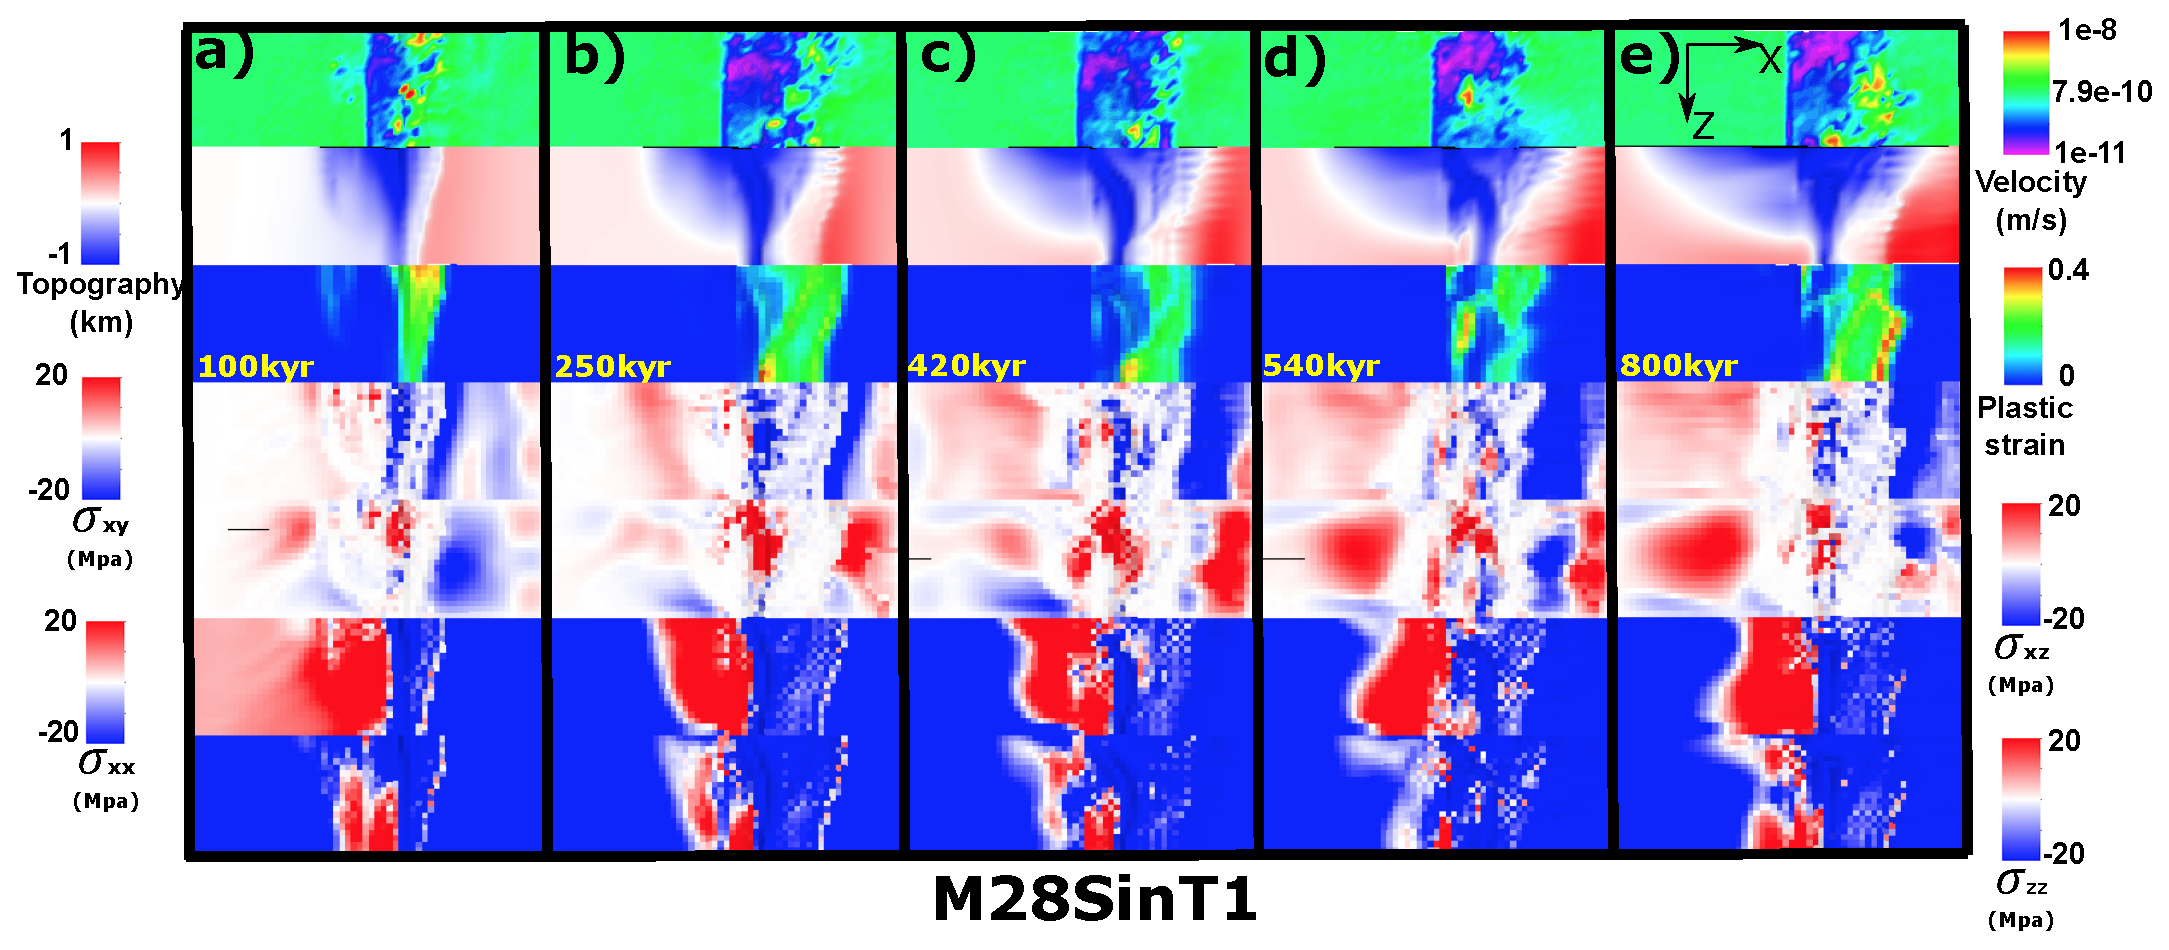
\includegraphics[width=1.0\textwidth]{./Figures/fig_Results_MRange_1_M28SinT1_time_evolution.eps}
 \caption{M28SinT1 (Table~\hyperref[Tab1_1]{\ref{Tab1_1}}) faulting and stress evolution with respect to time.}
\label{fig_Results_MRange_1}
\end{figure}

As shown in Figure~\hyperref[fig_Results_MRange_1]{\ref{fig_Results_MRange_1}}, faulting evolution is much less dynamic than that of M58SinT1. Faulting keeps on the right hand side of the ridge-axis. Only one secondary fault is formed at around 540kyr (Figure~\hyperref[fig_Results_MRange_1]{\ref{fig_Results_MRange_1}.d}). Initially, at 100kyr (Figure~\hyperref[fig_Results_MRange_1]{\ref{fig_Results_MRange_1}.a}), at the low Z side, the normal shear zone at conjugate plate takes up part of the extension and leave a dent in the topography. But it doesn't last long. The initial breakaway of the detachment extends further away from ridge-axis with four elements in along ridge-axis offset at 250kyr (Figure~\hyperref[fig_Results_MRange_1]{\ref{fig_Results_MRange_1}.b}). At 420kyr, at the high Z side, a hint of new near ridge-axis high angle normal fault begin to show up. It delvelop into a secondary fault at 540kyr (Figure~\hyperref[fig_Results_MRange_1]{\ref{fig_Results_MRange_1}.d}) and propagates toward high Z side. This results in a sinistral shear zone (red region in 5th row). At the low Z side (Z$=1\sim3$), a tensile failure can be seen and it take up part of the extension at the low Z side which results in the recede of termination at the low Z side as seen at 800kyr (Figure~\hyperref[fig_Results_MRange_1]{\ref{fig_Results_MRange_1}.e}) while the termination at higher Z side extends further away from the ridge-axis.

\subsubsection{M57SinT2 versus M58SinT2}
For description of M57SinT2 evolution with respect to time, please refer to Section~\hyperref[para_M57SinT2]{\ref{para_M57SinT2}} and Figure~\hyperref[fig_Results_Weakenging_4]{\ref{fig_Results_Weakenging_4}}. For description of M58SinT1 evolution with respect to time, please refer to  Section~\hyperref[para_M58SinT2]{\ref{para_M58SinT2}} and Figure~\hyperref[fig_Results_Weakenging_6]{\ref{fig_Results_Weakenging_6}}. A major difference is that M57SinT2 does not create alternating normal faults on each side of the ridge-axis while M58SinT2 does. \add[XT]{Why this seemingly small change could lead to such a to the first order difference in model behaviors?}

\subsubsection{M28LinT1 versus M57LinT1}
For description of M28LinT1 evolution with respect to time, please refer to Section~\hyperref[sec_M28LinT1]{\ref{sec_M28LinT1}}.
\paragraph{M57LinT1}\label{para_M57LinT1}

\begin{figure}[h]
 \centering
  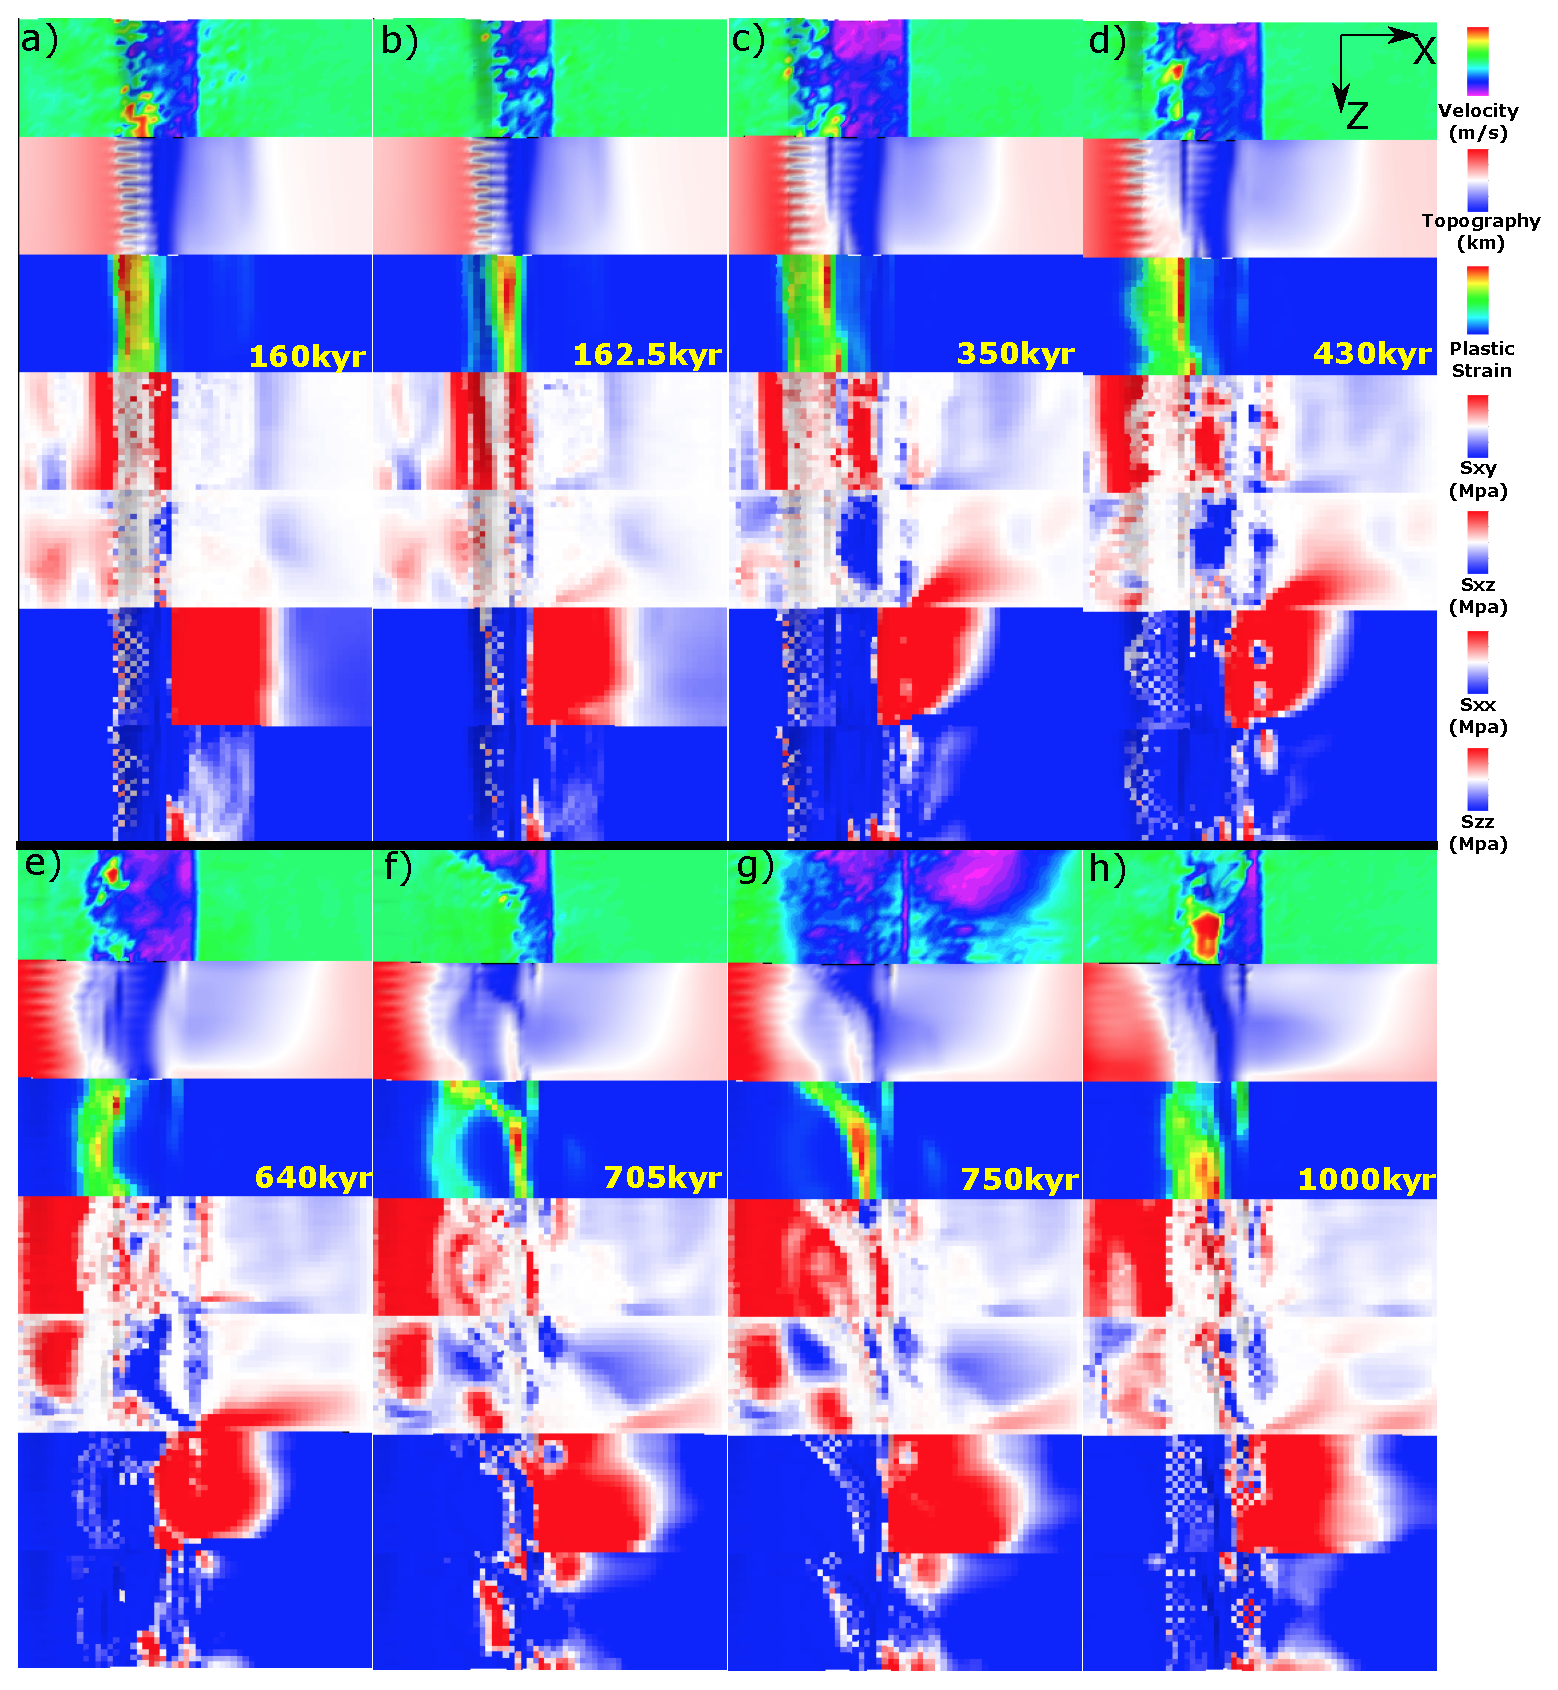
\includegraphics[width=0.8\textwidth]{./Figures/fig_Results_MRange_2_M57LinT1_time_evolution.eps}
 \caption{M57LinT1 (Table~\hyperref[Tab1_1]{\ref{Tab1_1}}) faulting and stress evolution with respect to time.}
\label{fig_Results_MRange_2}
\end{figure}

As shown in Figure~\hyperref[fig_Results_MRange_2]{\ref{fig_Results_MRange_2}}, between 160kyr (Figure~\hyperref[fig_Results_MRange_2]{\ref{fig_Results_MRange_2}.a}) and 162.5kyr (Figure~\hyperref[fig_Results_MRange_2]{\ref{fig_Results_MRange_2}.b}), there is a cut back. The corrugation is very severe and have a discrete distribution with one element width as its wavelength. The frontier of breakaway also shows discrete distribution of $\sigma_{xx}$ and $\sigma{zz}$ alternating between tension and compression which might be the reason for the undulating topography. At 350kyr (Figure~\hyperref[fig_Results_MRange_2]{\ref{fig_Results_MRange_2}.c} 3rd row), the two offsetted red line indicates tensile failure at the termination and the shorter one at the high Z side helps maintain a near ridge-axis high angle normal fault. At 430kyr (Figure~\hyperref[fig_Results_MRange_2]{\ref{fig_Results_MRange_2}.d}), the presence of vertical tensile failure near the ridge-axis at the low Z side is responsible for the recede of the front of the plastic strain at Z$=1\sim3$. While at Z=$5\sim10$, the breakaway keeps extending further away from the ridge-axis. This curved front results in a curved topography as seen in 640kyr (Figure~\hyperref[fig_Results_MRange_2]{\ref{fig_Results_MRange_2}.e}) and is also responsible for the large dextral shear (blue) zone (5th row). At 705kyr (Figure~\hyperref[fig_Results_MRange_2]{\ref{fig_Results_MRange_2}.f}), a new near ridge-axis secondary fault begin to evolve and replace the original one at high Z side with a length of $\sim15$ kilometers. The secondary fault also connect with the further away from ridge-axis original fault at low Z side. The topography at 1000kyr (Figure~\hyperref[fig_Results_MRange_2]{\ref{fig_Results_MRange_2}.h}) is a result of the curved and later connected fault. The frontier of the plastic strain at high Z side soon catch up with that at the low Z side due to the presence of a tensile failure zone a the low Z side that has taken up part of the extension.
       
\subsubsection{M28SqrtT1 versus M58SqrtT1}
For description of M28SqrtT1 evolution with respect to time, please refer to Paragraph~\hyperref[para_CutBack]{\ref{para_CutBack}} and Figure~\hyperref[fig_Results4_9]{\ref{fig_Results4_9}}.

For description of M58SqrtT1 evolution with respect to time, please refer to Paragraph~\hyperref[para_M58SqrtT1]{\ref{para_M58SqrtT1}} and Figure~\hyperref[fig_Results_Weakenging_7]{\ref{fig_Results_Weakenging_7}}.


\subsubsection{M57SqrtT2 versus M58SqrtT2}

For description of M58SqrtT2 evolution with respect to time, please refer to Paragraph~\hyperref[para_M58SqrtT2]{\ref{para_M58SqrtT2}} and Figure~\hyperref[fig_Results_Weakenging_8]{\ref{fig_Results_Weakenging_8}}.

The major difference between M57SqrtT2 and M58SqrtT2 is that M57SqrtT2 keeps faulting at the same side of the ridge-axis while M58SqrtT2 alternates.

\paragraph{M57SqrtT2}

\begin{figure}[h]
 \centering
  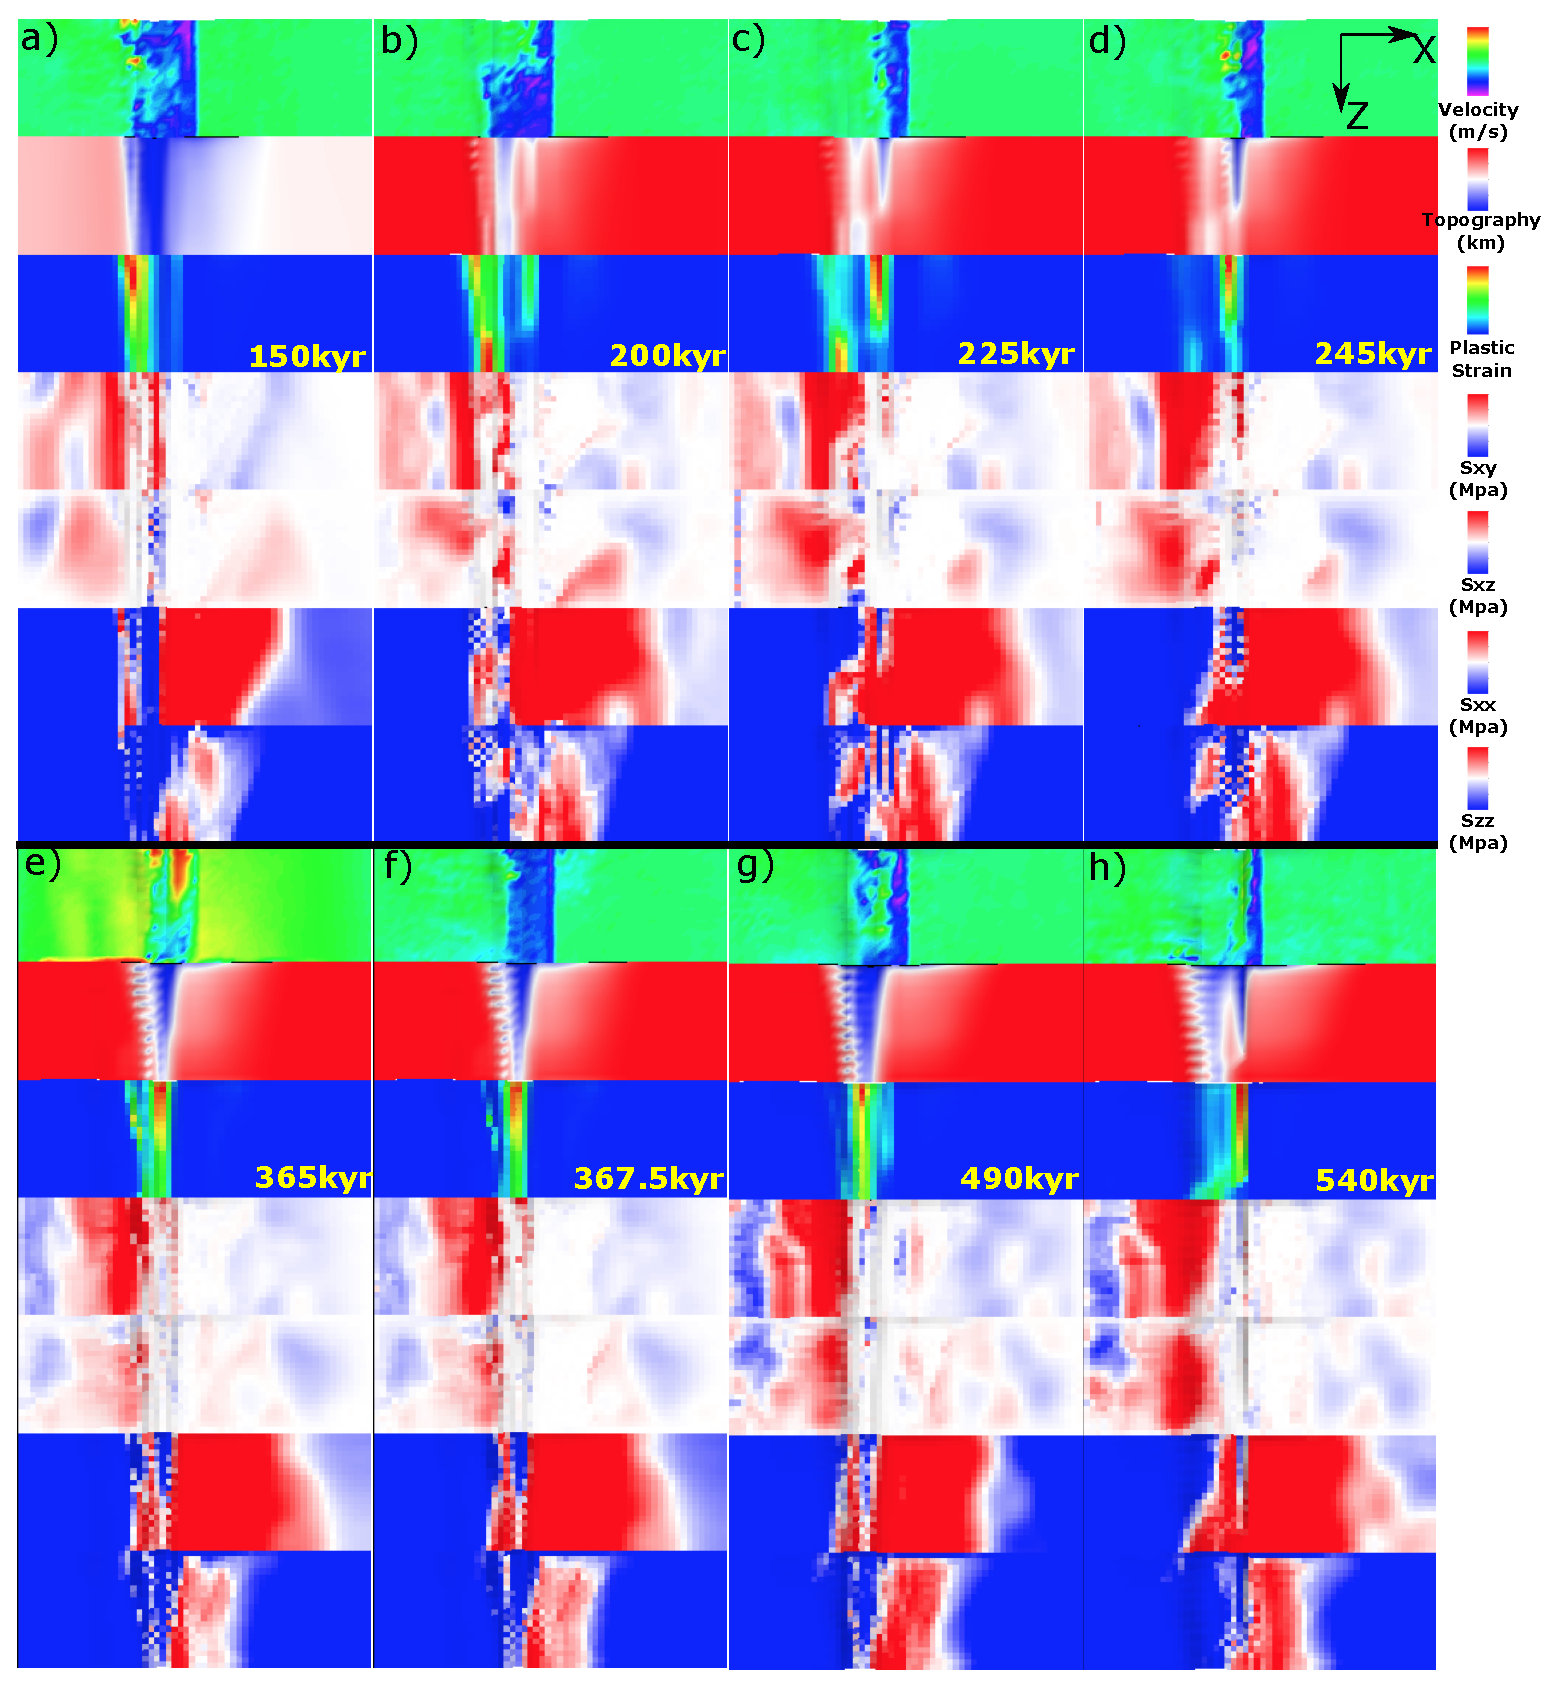
\includegraphics[width=0.8\textwidth]{./Figures/fig_Results_MRange_3_M57SqrtT2_time_evolution.eps}
 \caption{M57SqrtT2 (Table~\hyperref[Tab1_1]{\ref{Tab1_1}}) faulting and stress evolution with respect to time.}
\label{fig_Results_MRange_3}
\end{figure}

For M57SqrtT2, there are totally six small scale cut back happen at 282.5kyr, 290kyr, 365kyr, 452.5kyr, 482.5kyr and 540kyr respectively (the model stops at 540kyr). As shown in Figure~\hyperref[fig_Results_MRange_3]{\ref{fig_Results_MRange_3}}, the fault keeps on the left hand side of the ridge-axis. At 200kyr (Figure~\hyperref[fig_Results_MRange_3]{\ref{fig_Results_MRange_3}.b}), a new near ridge-axis high angle normal fault begin to evolve and take the place of the initial one. As the fault evolve, a transient stage of discontinuous abyssal hill is produced at the low Z side as seen at 225kyr (Figure~\hyperref[fig_Results_MRange_3]{\ref{fig_Results_MRange_3}.c}). The fault propagate toward high Z side and cut through the plate at $\sim$245kyr (Figure~\hyperref[fig_Results_MRange_3]{\ref{fig_Results_MRange_3}.d}) when sawtooth shape topography at the low Z side (2nd row) is created by sawtooth shape $\sigma_{xx}$ (6th row) and $\sigma_{zz}$ (7th row). Between 365kyr (Figure~\hyperref[fig_Results_MRange_3]{\ref{fig_Results_MRange_3}.e}) and 367.5kyr (Figure~\hyperref[fig_Results_MRange_3]{\ref{fig_Results_MRange_3}.f}), there is a cut back. At 490kyr (Figure~\hyperref[fig_Results_MRange_3]{\ref{fig_Results_MRange_3}.g}), there is new near ridge-axis antithetic fault on the hanging wall which terminates the old fault and develops into a vertical near ridge-axis tensile failure as seen at 540kyr (Figure~\hyperref[fig_Results_MRange_3]{\ref{fig_Results_MRange_3}.h}).

\subsection{Cut-back}

\subsection{Corrugations}
\subsubsection{Corrugations due to anastomosing}
\subsubsection{Corrugations due to asynchronous normal faulting}

\subsection{Summary of Results}
There are several behaviors that are controlled by the model parameters. Generally, only M58 models with Type two weakening produce aternating faults on both side of the ridge-axis. All the models show corrugations. As for faulting patterns in terms of evolution frequency, usually Square root is more dynamic than Sinusoidal than Linear, M58 is more dynamic than M57 than M28.

Following tables are a summery of the model behaviors with respect to different setup parameters.
 

\begin{table}[h]
\begin{small}
\begin{center}
\begin{tabular}{||l|l||l|l||l|l||}
\hline
A & Alternating Fault & C & Corrugation & SL & Shear Topography Low \\
\hline
NA& Not Alternating & SF & Secondary Fault on one side & CB & Cut Back   \\
\hline
DD &  Double Dome  & AM    & Atlantis Massif Shape &  &   \\
\hline
\end{tabular}
\end{center}
\end{small}
\caption{Model behaviors in short.}
\label{Tab1}
\end{table}

Based on the 11 models with M variation, we observed eight first-order behaviors as shown in Table~\hyperref[Tab1]{\ref{Tab1}}. 


\begin{table}[h]
\begin{small}
\begin{center}
\begin{tabular}{|l|p{3.5cm}|p{3.5cm}|p{3.5cm}|}
\hline
\diagbox[width=6em]{Type}{M range}&
M28&M57&M58\\
\hline
Type one &NA; C; SL; SF$_{1500kyr}$; DD    &NA; C; SF$_{1380kyr}$; CB$_{330kyr}$; AM(opposite z)     &    \\
\hline
Type two &    &     &    \\
\hline
\end{tabular}
\end{center}
\end{small}
\caption{Linear functional form.}
\end{table}

\begin{center}
\begin{table}[h!]
\begin{small}
\begin{tabular}{|l|p{3.5cm}|p{3.5cm}|p{3.5cm}|}
\hline
\diagbox[width=6em]{Type}{M range}&
M28&M57&M58\\
\hline
Type one & NA; C; SL; SF$_{995kyr}$ & NA; C; SL; SF$_{760kyr;1320kyr}$; CB$_{520kyr}$; AM & NA; C; SL; CB$_{510kyr}$; SF$_{760kyr;1140kyr;1990kyr}$   \\
\hline
Type two &    &NA; C; SL; SF$_{680kyr}$; CB$_{905kyr}$     & A$_{450kyr;600kyr}$; C(only at low M); CB$_{990kyr}$   \\
\hline
\end{tabular}
\end{small}
\caption{Sinusoidal functional form.}
\end{table}
\end{center}

\begin{table}[ht]
\begin{small}
\begin{center}
\begin{tabular}{|l|p{3.5cm}|p{3.5cm}|p{3.5cm}|}
\hline
\diagbox[width=6em]{Type}{M range}&
M28&M57&M58\\
\hline
Type one & NA; C; SL; CB$_{205kyr;330kyr;1025kyr}$   &      & NA; C$_{1770kyr}$(due to shear with dif wave length); SF$_{860kyr}$(high M); SF$_{1190kyr}$(low M)(Dog Bone); SF$_{1690kyr}$    \\
\hline
Type two &    & NA; C; SF$_{435kyr;1060kyr}$; CB$_{585kyr}$; CB$_{735kyr}$; CB$_{910kyr}$; CB$_{970kyr}$    & A$_{550kyr;920kyr}$; C; CB$_{400kyr}$    \\
\hline
\end{tabular}
\end{center}
\end{small}
\caption{Square root functional form.}
\end{table}
